\documentclass[12pt,a4paper]{article}
\usepackage[T2A]{fontenc}
\usepackage[utf8]{inputenc}
\usepackage[russian]{babel}
\usepackage{geometry}
\geometry{top=2cm, bottom=2cm, left=2cm, right=1.5cm}
\usepackage{graphicx}
\usepackage{amsmath}
\usepackage{amssymb}
\usepackage{float}
\usepackage{caption}
\usepackage{hyperref}
\usepackage{enumitem}
\setlist[itemize]{leftmargin=*}
\setlist[enumerate]{leftmargin=*}

% \title{\textbf{Отчёт по лабораторной работе:} \\ Исследование дифракции света}
% \author{ФИО студента \\ Группа: \_\_\_\_\_\_\_\_\_\_}
% \date{\today}

\begin{document}
\title{\begin{center}Лабораторная работа №4.3.1:\end{center}
Изучение дифракции света}
\author{Струков О. И. \\ Б04-404}
\date{}

\thispagestyle{empty}
\pagenumbering{gobble}
\maketitle
\newpage
\pagenumbering{arabic}

\section*{Теоретическая часть}
Дифракцией называется волновое явление, проявляющееся в отклонении распространения света от законов геометрической оптики при наличии препятствий или неоднородностей среды. Математическое описание дифракции основано на принципе Гюйгенса-Френеля, согласно которому каждый элемент волнового фронта рассматривается как источник вторичных сферических волн, а результирующее световое поле формируется в результате их интерференции.

Для расчёта распределения интенсивности в ближней волновой зоне применяется метод зон Френеля. Открытая часть волнового фронта разбивается на концентрические кольцевые зоны таким образом, чтобы разность хода от краёв соседних зон до точки наблюдения составляла $\lambda/2$. Радиус $m$-й зоны Френеля определяется выражением:
\begin{equation}
r_m = \sqrt{m \lambda z},
\end{equation}
где $\lambda$ -- длина волны излучения, $z$ -- расстояние от апертуры до плоскости наблюдения. Суммирование вкладов от зон удобно выполнять с помощью векторных диаграмм, приводящих к построению спирали Френеля. Характер дифракционной картины определяется волновым параметром $p = \sqrt{\lambda z}/r = 1/\sqrt{N}$, где $N$ --- число открытых зон. Выделяются три режима: геометрическая оптика ($p \ll 1$), дифракция Френеля ($p \sim 1$) и дифракция Фраунгофера ($p \gg 1$).

При дифракции на щели радиальная симметрия теряется, и метод векторных диаграмм приводит к спирали Корню. Открытая часть волнового фронта разбивается на прямоугольные зоны Шустера с координатами $\xi_m = \sqrt{m\lambda z}$. Суммирование вкладов от зон $\xi > 0$ и $\xi < 0$ даёт результирующий вектор, соединяющий соответствующие точки на спирали Корню. При чётном числе открытых зон наблюдается минимум интенсивности, при нечётном --- максимум. Для описания дифракции на непрозрачных препятствиях применяется принцип Бабине, согласно которому сумма амплитуд полей, дифрагировавших на дополнительном экране и на исходном экране, равна амплитуде поля при отсутствии препятствий.

В дальней волновой зоне ($p \gg 1$) реализуется дифракция Фраунгофера. Для локализации картины используется линза, фокусирующая параллельные лучи в свою фокальную плоскость. При дифракции плоской волны на щели ширины $b$ распределение интенсивности описывается выражением:
\begin{equation}
I(\theta) = I(0) \left( \frac{\sin\left( \frac{k b \sin\theta}{2} \right)}{\frac{k b \sin\theta}{2}} \right)^2, \quad k = \frac{2\pi}{\lambda}.
\end{equation}
Минимумы интенсивности наблюдаются при углах, удовлетворяющих условию $b \sin\theta = m\lambda$. В фокальной плоскости линзы с фокусным расстоянием $f$ координаты минимумов задаются формулой:
\begin{equation}
x_m = f \frac{m \lambda}{b}, \quad m = \pm 1, \pm 2, \dots
\end{equation}
Ширина центрального дифракционного максимума обратно пропорциональна ширине щели. При смещении апертуры в плоскости, перпендикулярной оптической оси, положение дифракционной картины не изменяется, так как угловое распределение определяется только геометрией препятствия и длиной волны.

\begin{figure}[H]
    \centering
    
\includegraphics[width=0.6\textwidth]{1.jpg}
    \caption{Спираль Френеля.}
    \label{fig:fresnel}
\end{figure}

\begin{figure}[H]
    \centering
    
\includegraphics[width=0.5\textwidth]{2.jpg}
    \caption{Спираль Корню и зоны Шустера для дифракции на щели.}
    \label{fig:cornu}
\end{figure}

\begin{figure}[H]
    \centering
    
\includegraphics[width=0.6\textwidth]{3.jpg}
    \caption{Распределение амплитуды колебаний и интенсивности излучения, полученное в 
фокальной плоскости линзы с фокусным расстоянием f при дифракции Фраунгофера на щели ширины b.}
    \label{fig:fraunhofer}
\end{figure}















\newpage
\section*{Ход работы}
\subsection*{I. Дифракция Френеля}

Оптическая схема была собрана согласно рис.~4. Источник света, щель $d_1$, линза $l_1$, щель $d_2$ и микроскоп были последовательно установлены на оптической скамье и отцентрированы. Щель $d_2$ размещалась на минимальном расстоянии от линзы $l_1$.
\begin{figure}[H]
    \centering
    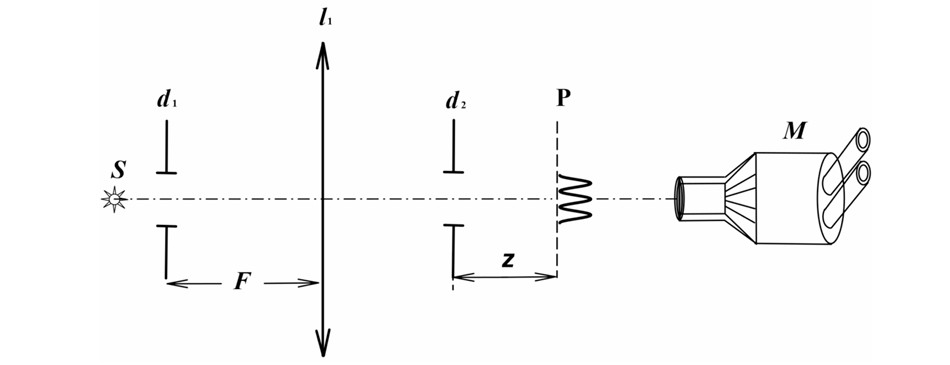
\includegraphics[width=0.7\textwidth]{4.jpg}
    \caption{Схема установки для наблюдения дифракции Френеля.}
    % \label{fig:cornu}
\end{figure}
Микроскоп был сфокусирован на щель $d_2$ для получения резкого геометрического изображения. Яркость источника света была настроена таким образом, чтобы избежать засвечивания изображения.

При отодвигании микроскопа от щели на фоне геометрического изображения были наблюдены узкие тёмные дифракционные полосы, появляющиеся сначала у краёв щели.% Контрастность картины была оптимизирована подбором ширины щели $d_1$ и яркости источника.
Была снята зависимость координаты микроскопа z от количества наблюдаемых тёмных полос n (нулю сопоставлена координата, в которой щель видна максимально резко):

% \textbf{Результаты измерений:}

% \begin{itemize}
%     \item Начальная координата микроскопа (резкое изображение щели): $z_0 = $\_\_\_\_\_\_\_~мм
%     \item Положение микроскопа при наблюдении одной тёмной полосы ($n=1$): $z_1 = $\_\_\_\_\_\_\_~мм
%     \item Расстояние от щели до плоскости наблюдения при $n=1$: $z = z_1 - z_0 = $\_\_\_\_\_\_\_~мм
%     \item Измерена зависимость координаты $z$ от числа наблюдаемых тёмных полос $n$:
% \end{itemize}

\begin{table}[H]
\centering
\begin{tabular}{|c|c|}
\hline
$n$ & $z$, см \\
\hline
0 & 0  \\\hline
1 & 6,9  \\\hline
2 & 4,0  \\\hline
3 & 2,9  \\\hline
4 & 2,3  \\\hline
5 & 1,9  \\\hline
6 & 1,65  \\
\hline
\end{tabular}
\caption{Зависимость расстояния $z$ от числа тёмных полос $n$}

\end{table}

Ширина щели $d_2$ была определена двумя методами:
\begin{itemize}
    \item По микрометрическому винту: $b_{\text{мкр}} \sim $ 300 мкм.
    \item Прямым измерением геометрического изображения на экране: $b_{\text{экр}} =  (475,7 \pm 5)$ мкм.
\end{itemize}



% \textbf{Обработка результатов:}

Поскольку зависимость z(n) описывается формулой $z = \dfrac{b^2}{2\lambda(n+1)}$, для нахождения ширины щели был построен график зависимости $z(1/(n+1))$:
% Построен график зависимости $1/z(m)$ (рис.~\ref{fig:fresnel_z_m}).

\begin{figure}[H]
    \centering
    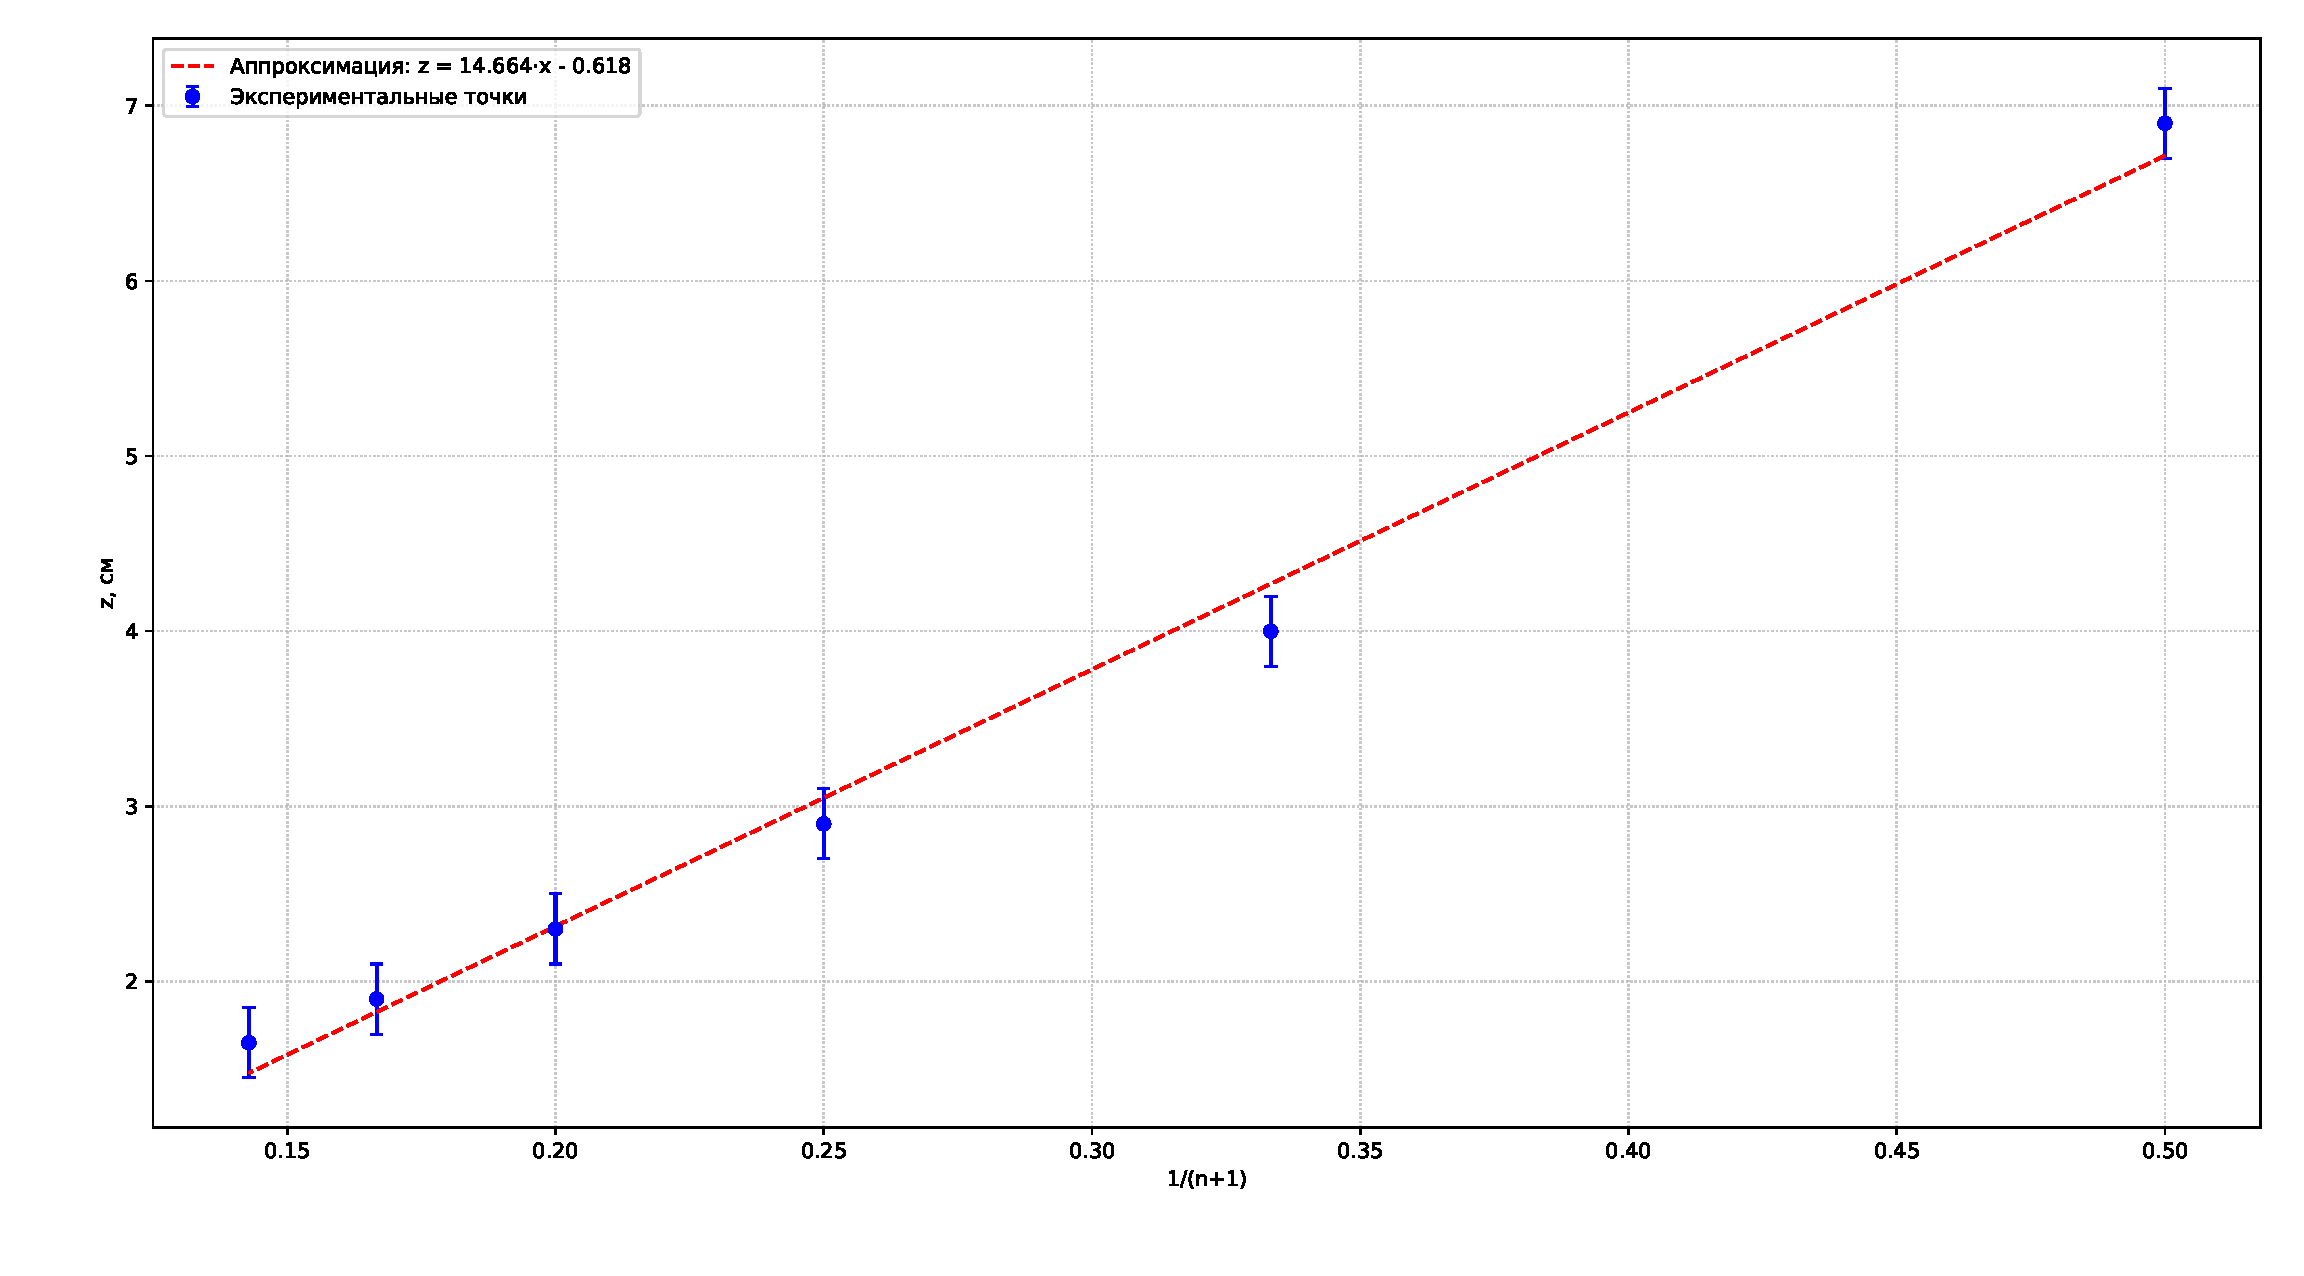
\includegraphics[width=0.8\textwidth]{zn.pdf}
    \caption{График зависимости $z(1/(n+1))$.}
    \label{fig:fresnel_z_m}
\end{figure}

По наклону прямой была определена ширина щели ($\lambda \approx 555$ нм): $b_{\text{граф}} = (403 \pm 20)$ мкм, что близко к результатам, полученным ранее, но не совпадает с ними в пределах погрешностей.


% Результаты сравнения:
% \begin{itemize}
%     \item $b_{\text{граф}} = $\_\_\_\_\_\_\_~мкм
%     \item $b_{\text{мкр}} = $\_\_\_\_\_\_\_~мкм
%     \item Расхождение: \_\_\_\_\_\_\_\%
% \end{itemize}

Построен качественный график распределения интенсивности на границе света и тени при дифракции на краю экрана (рис.~\ref{fig:cornu_intensity}).

\begin{figure}[H]
    \centering
    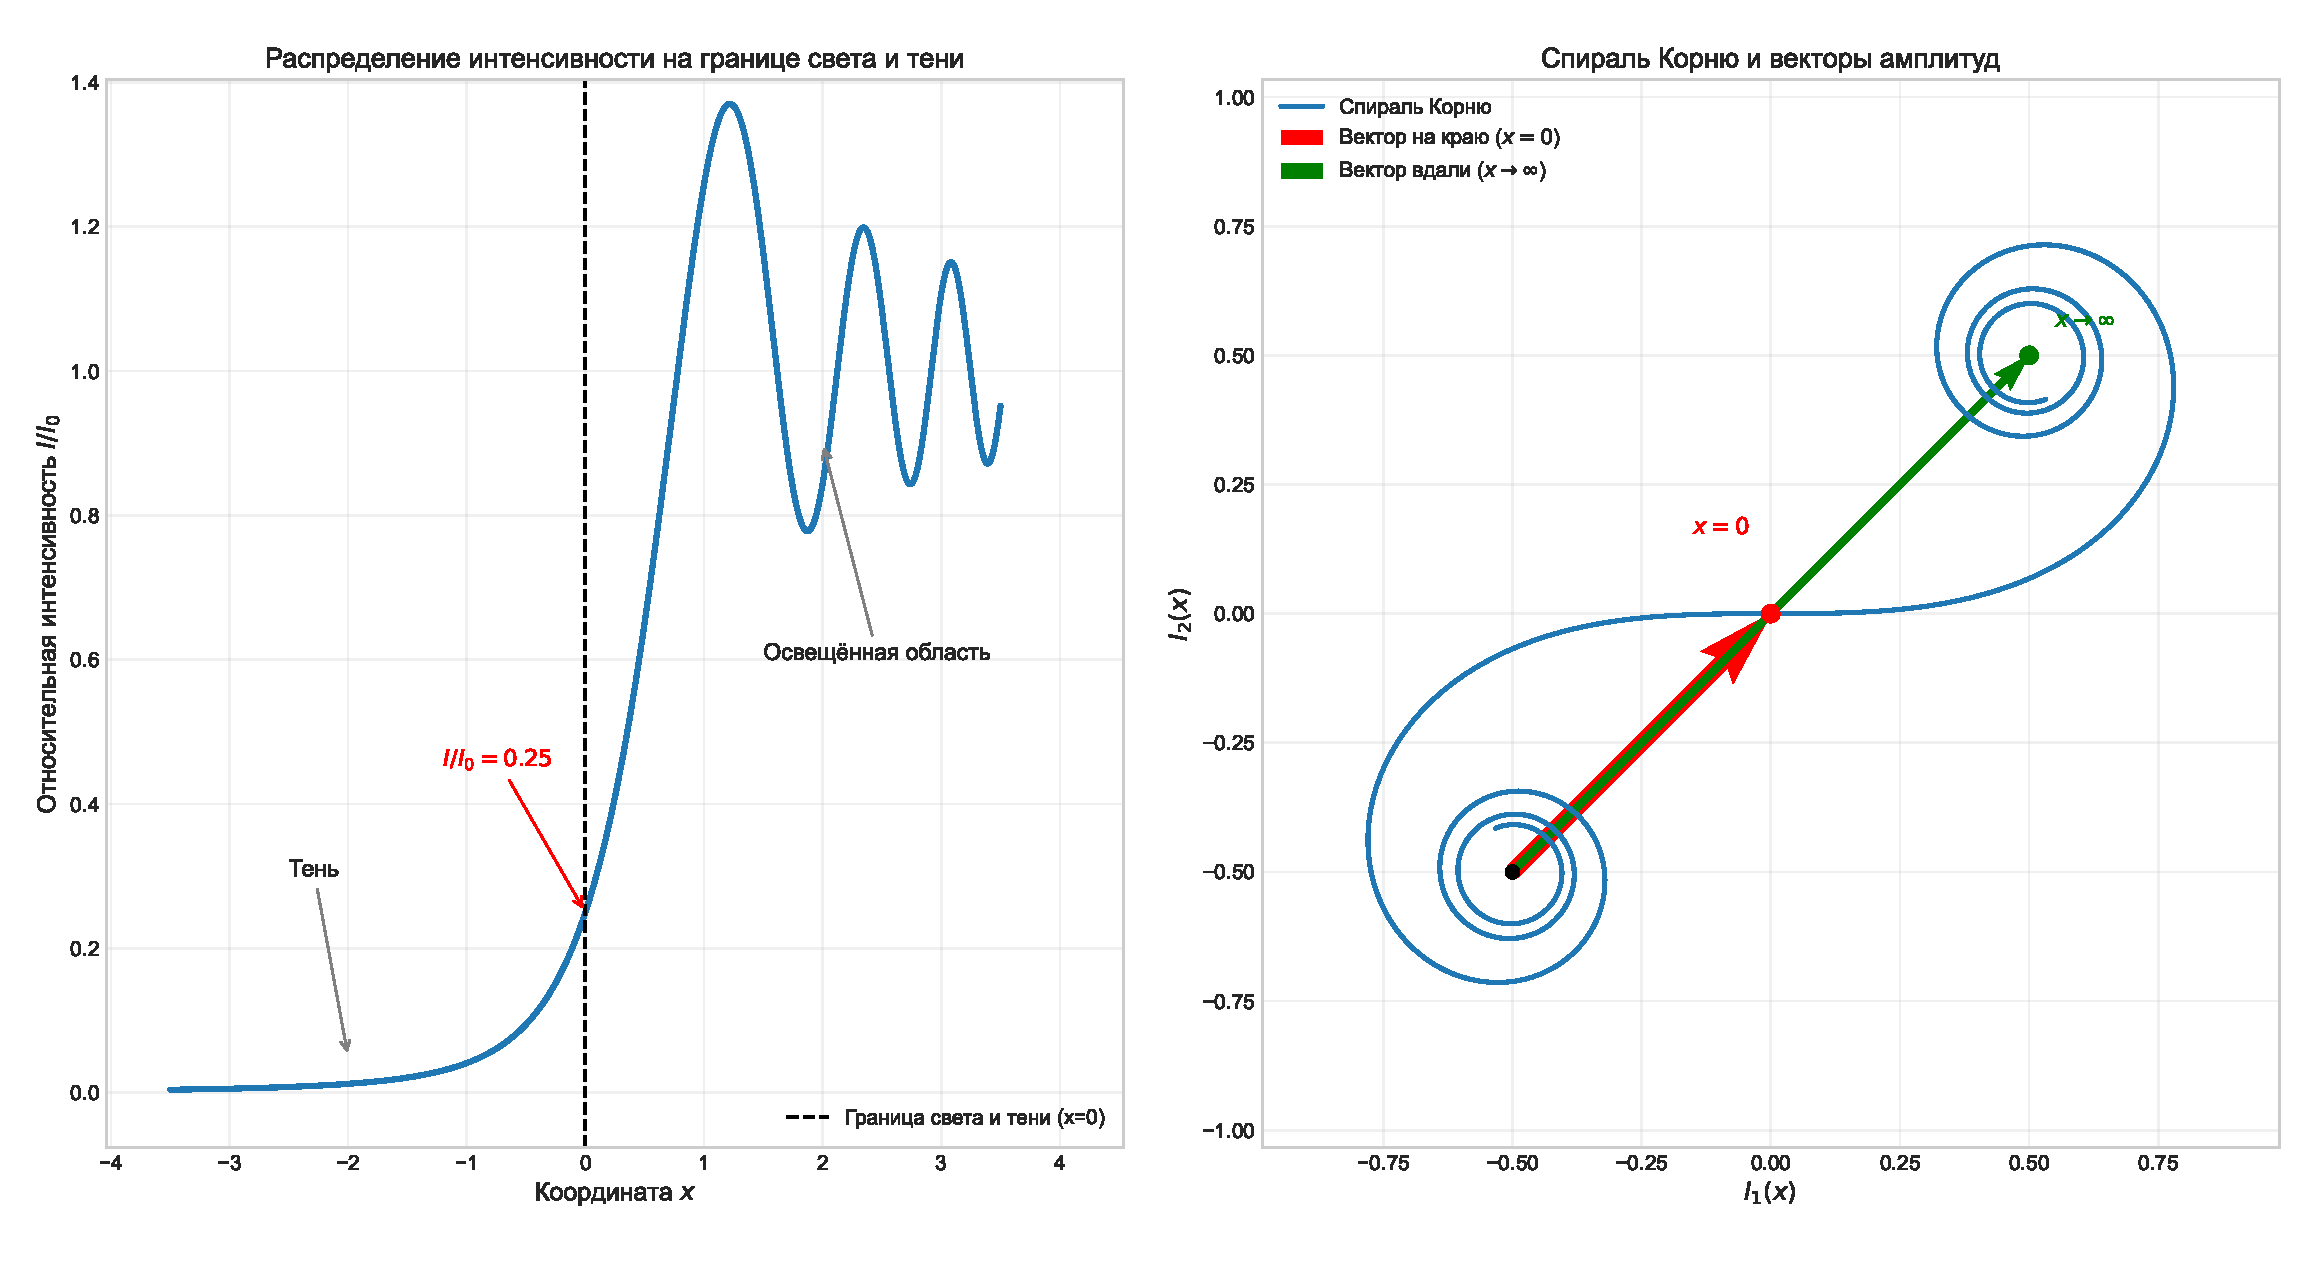
\includegraphics[width=0.8\textwidth]{I.pdf}
    \caption{Распределение интенсивности на границе света и тени.}
    \label{fig:cornu_intensity}
\end{figure}

По спирали Корню видно, что интенсивность света на самой границе геометрической тени составляет одну четверть от интенсивности вдали от экрана в освещённой области, так как амплитуда колебаний на краю соответствует половине вектора напряжённости для полностью открытого фронта.

% Видимое число тёмных полос связано с шириной щели соотношением $b = (\sqrt{m_1} + \sqrt{m_2})\sqrt{\lambda z}$, где $m_1$ и $m_2$ -- числа открытых зон Шустера для положительной и отрицательной частей щели. При увеличении ширины щели увеличивается число открывающихся зон, что приводит к появлению дополнительных тёмных полос в дифракционной картине.

\textbf{Качественные наблюдения:}

\begin{itemize}
    \item При небольшом удалении микроскопа от щели у её краёв наблюдались узкие частые полосы (дифракция на краю экрана). Возле границы щели располагалась самая яркая светлая полоса (рис. 7).
    
    \item При уменьшении ширины щели $d_2$ изображение становилось уже, а дифракционных полос в центре становилось больше (рис. 7-8),
    поскольку видимое число тёмных полос связано с шириной щели соотношением $b = (\sqrt{m_1} + \sqrt{m_2})\sqrt{\lambda z}$, где $m_1$ и $m_2$ -- числа открытых зон Шустера для положительной и отрицательной частей щели. При увеличении ширины щели увеличивается число открывающихся зон, что приводит к появлению дополнительных тёмных полос в дифракционной картине.


    \begin{figure}[H]
    \centering
    \begin{minipage}{0.45\textwidth}
        \centering
        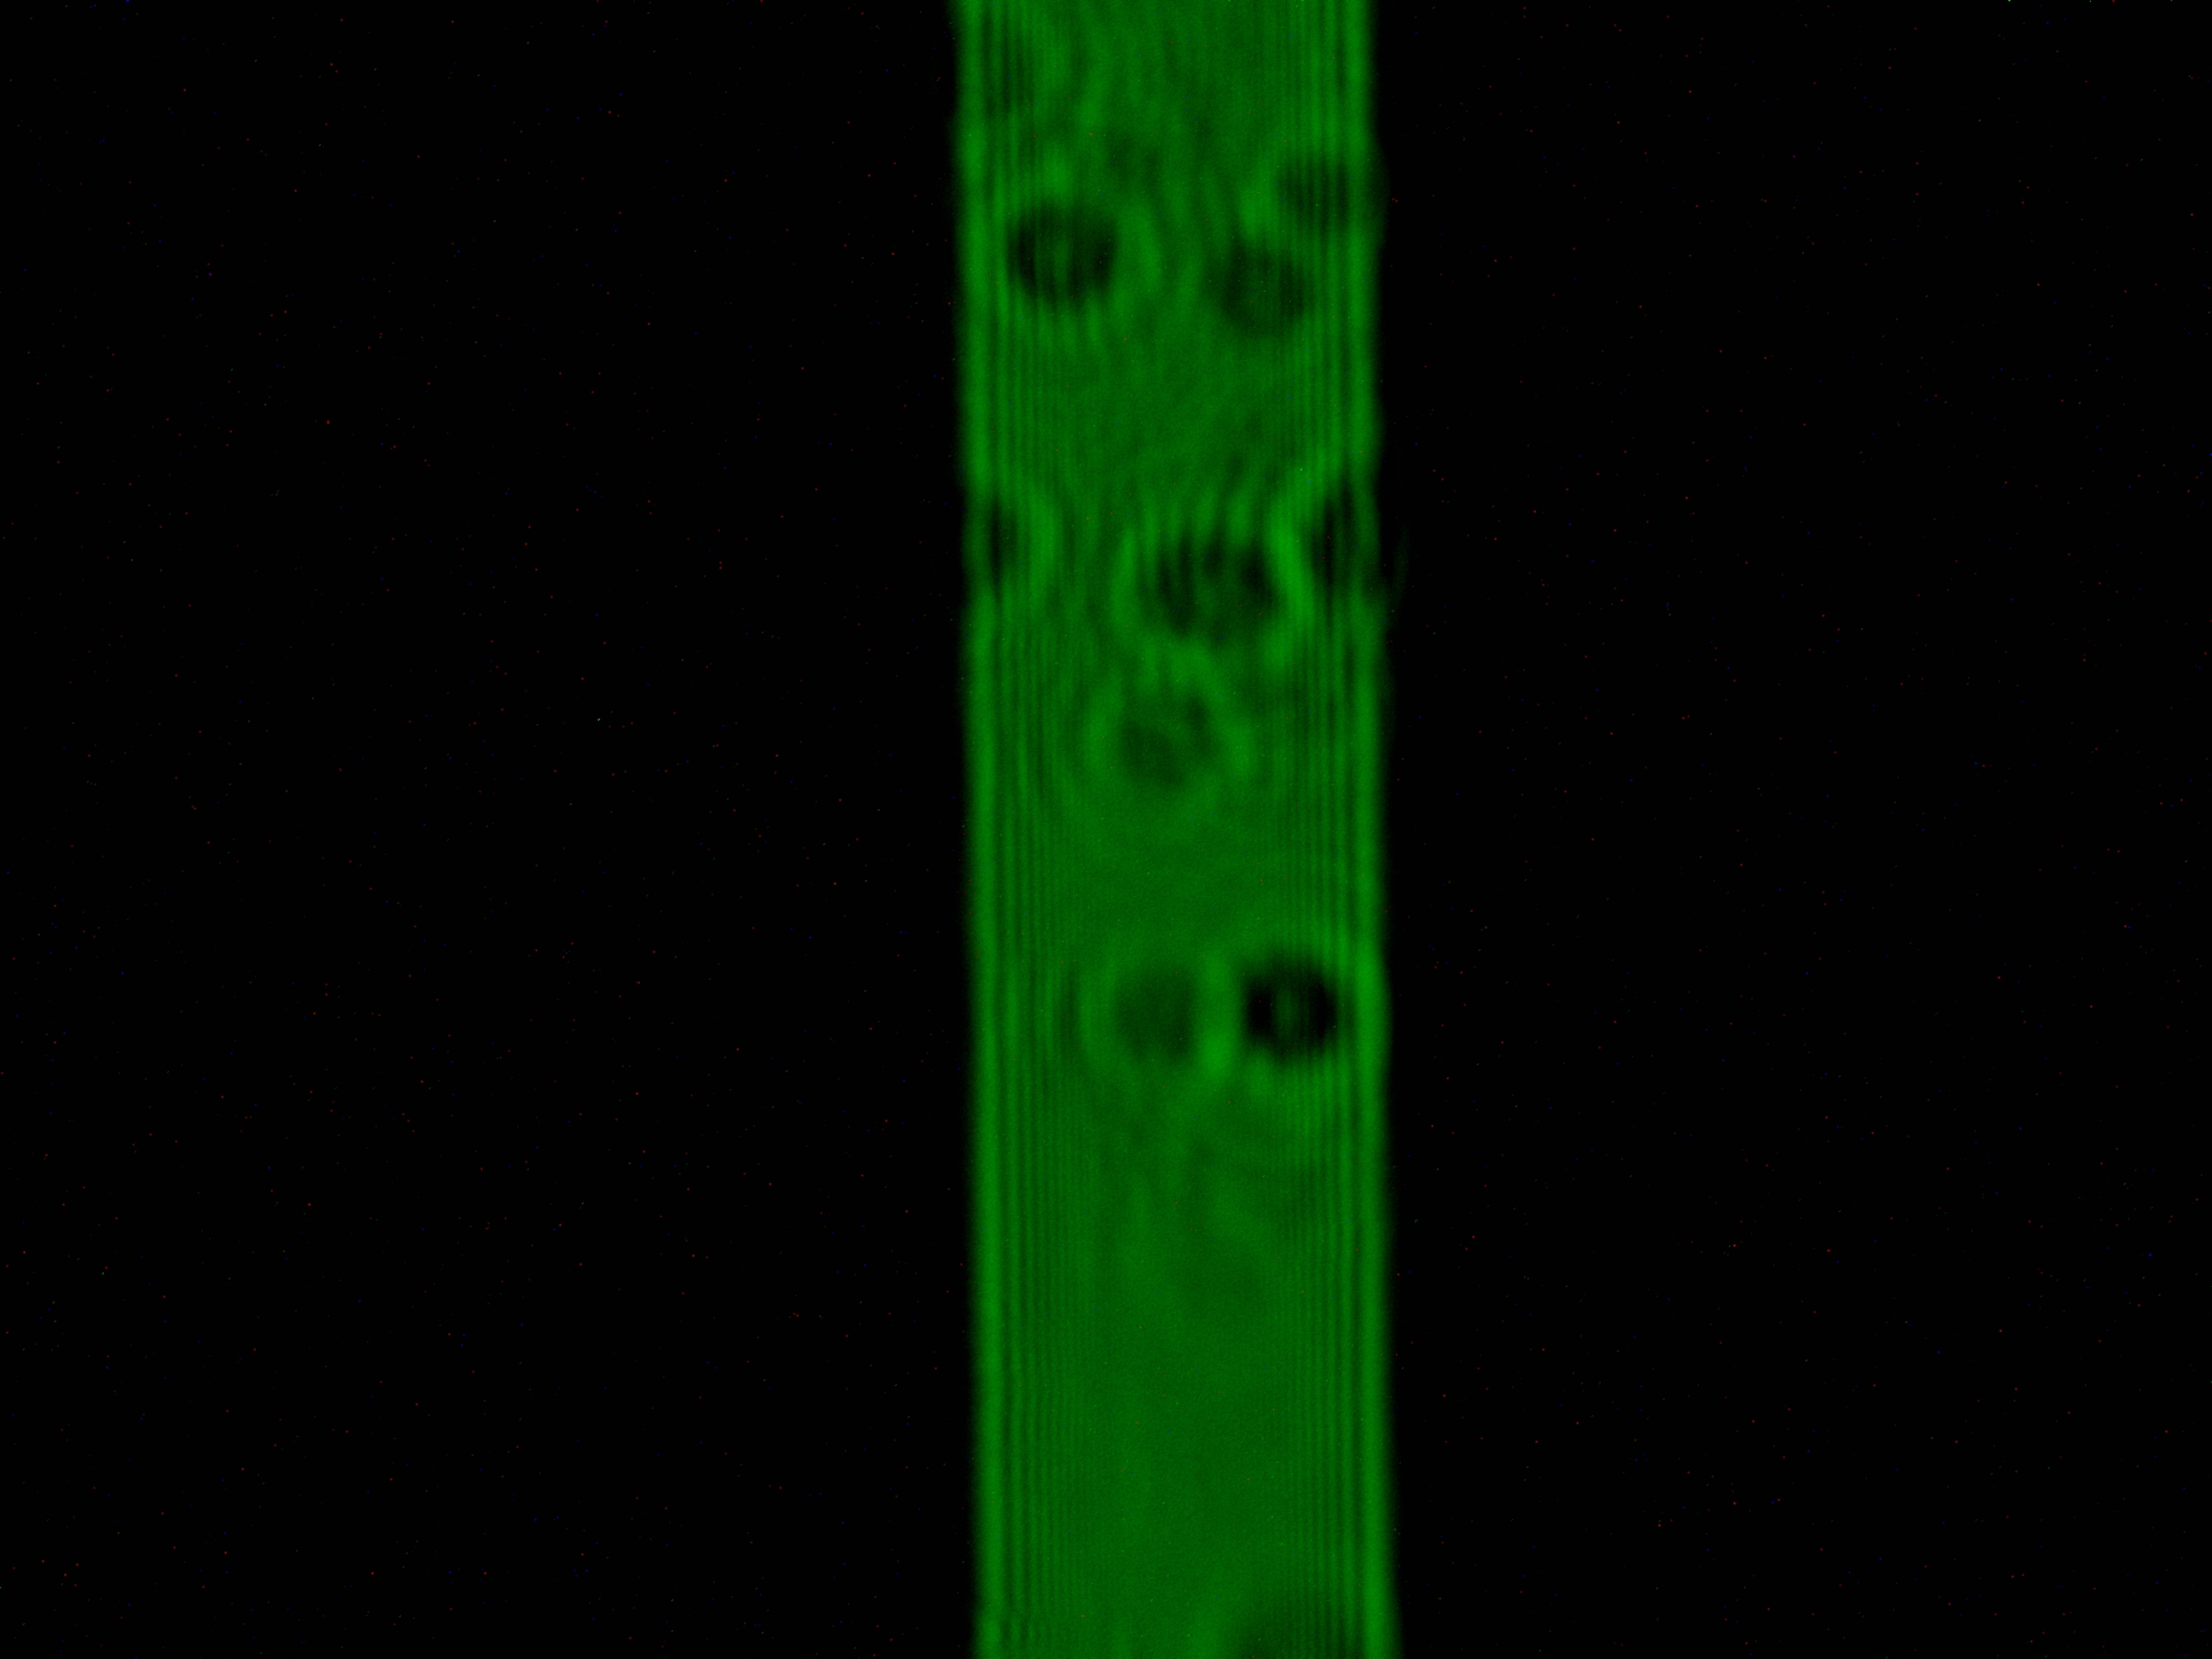
\includegraphics[width=\textwidth]{Фото/1.11.jpg}
        \caption{$d_2$ открыта пошире.}
    \end{minipage}\hfill
    \begin{minipage}{0.45\textwidth}
        \centering
        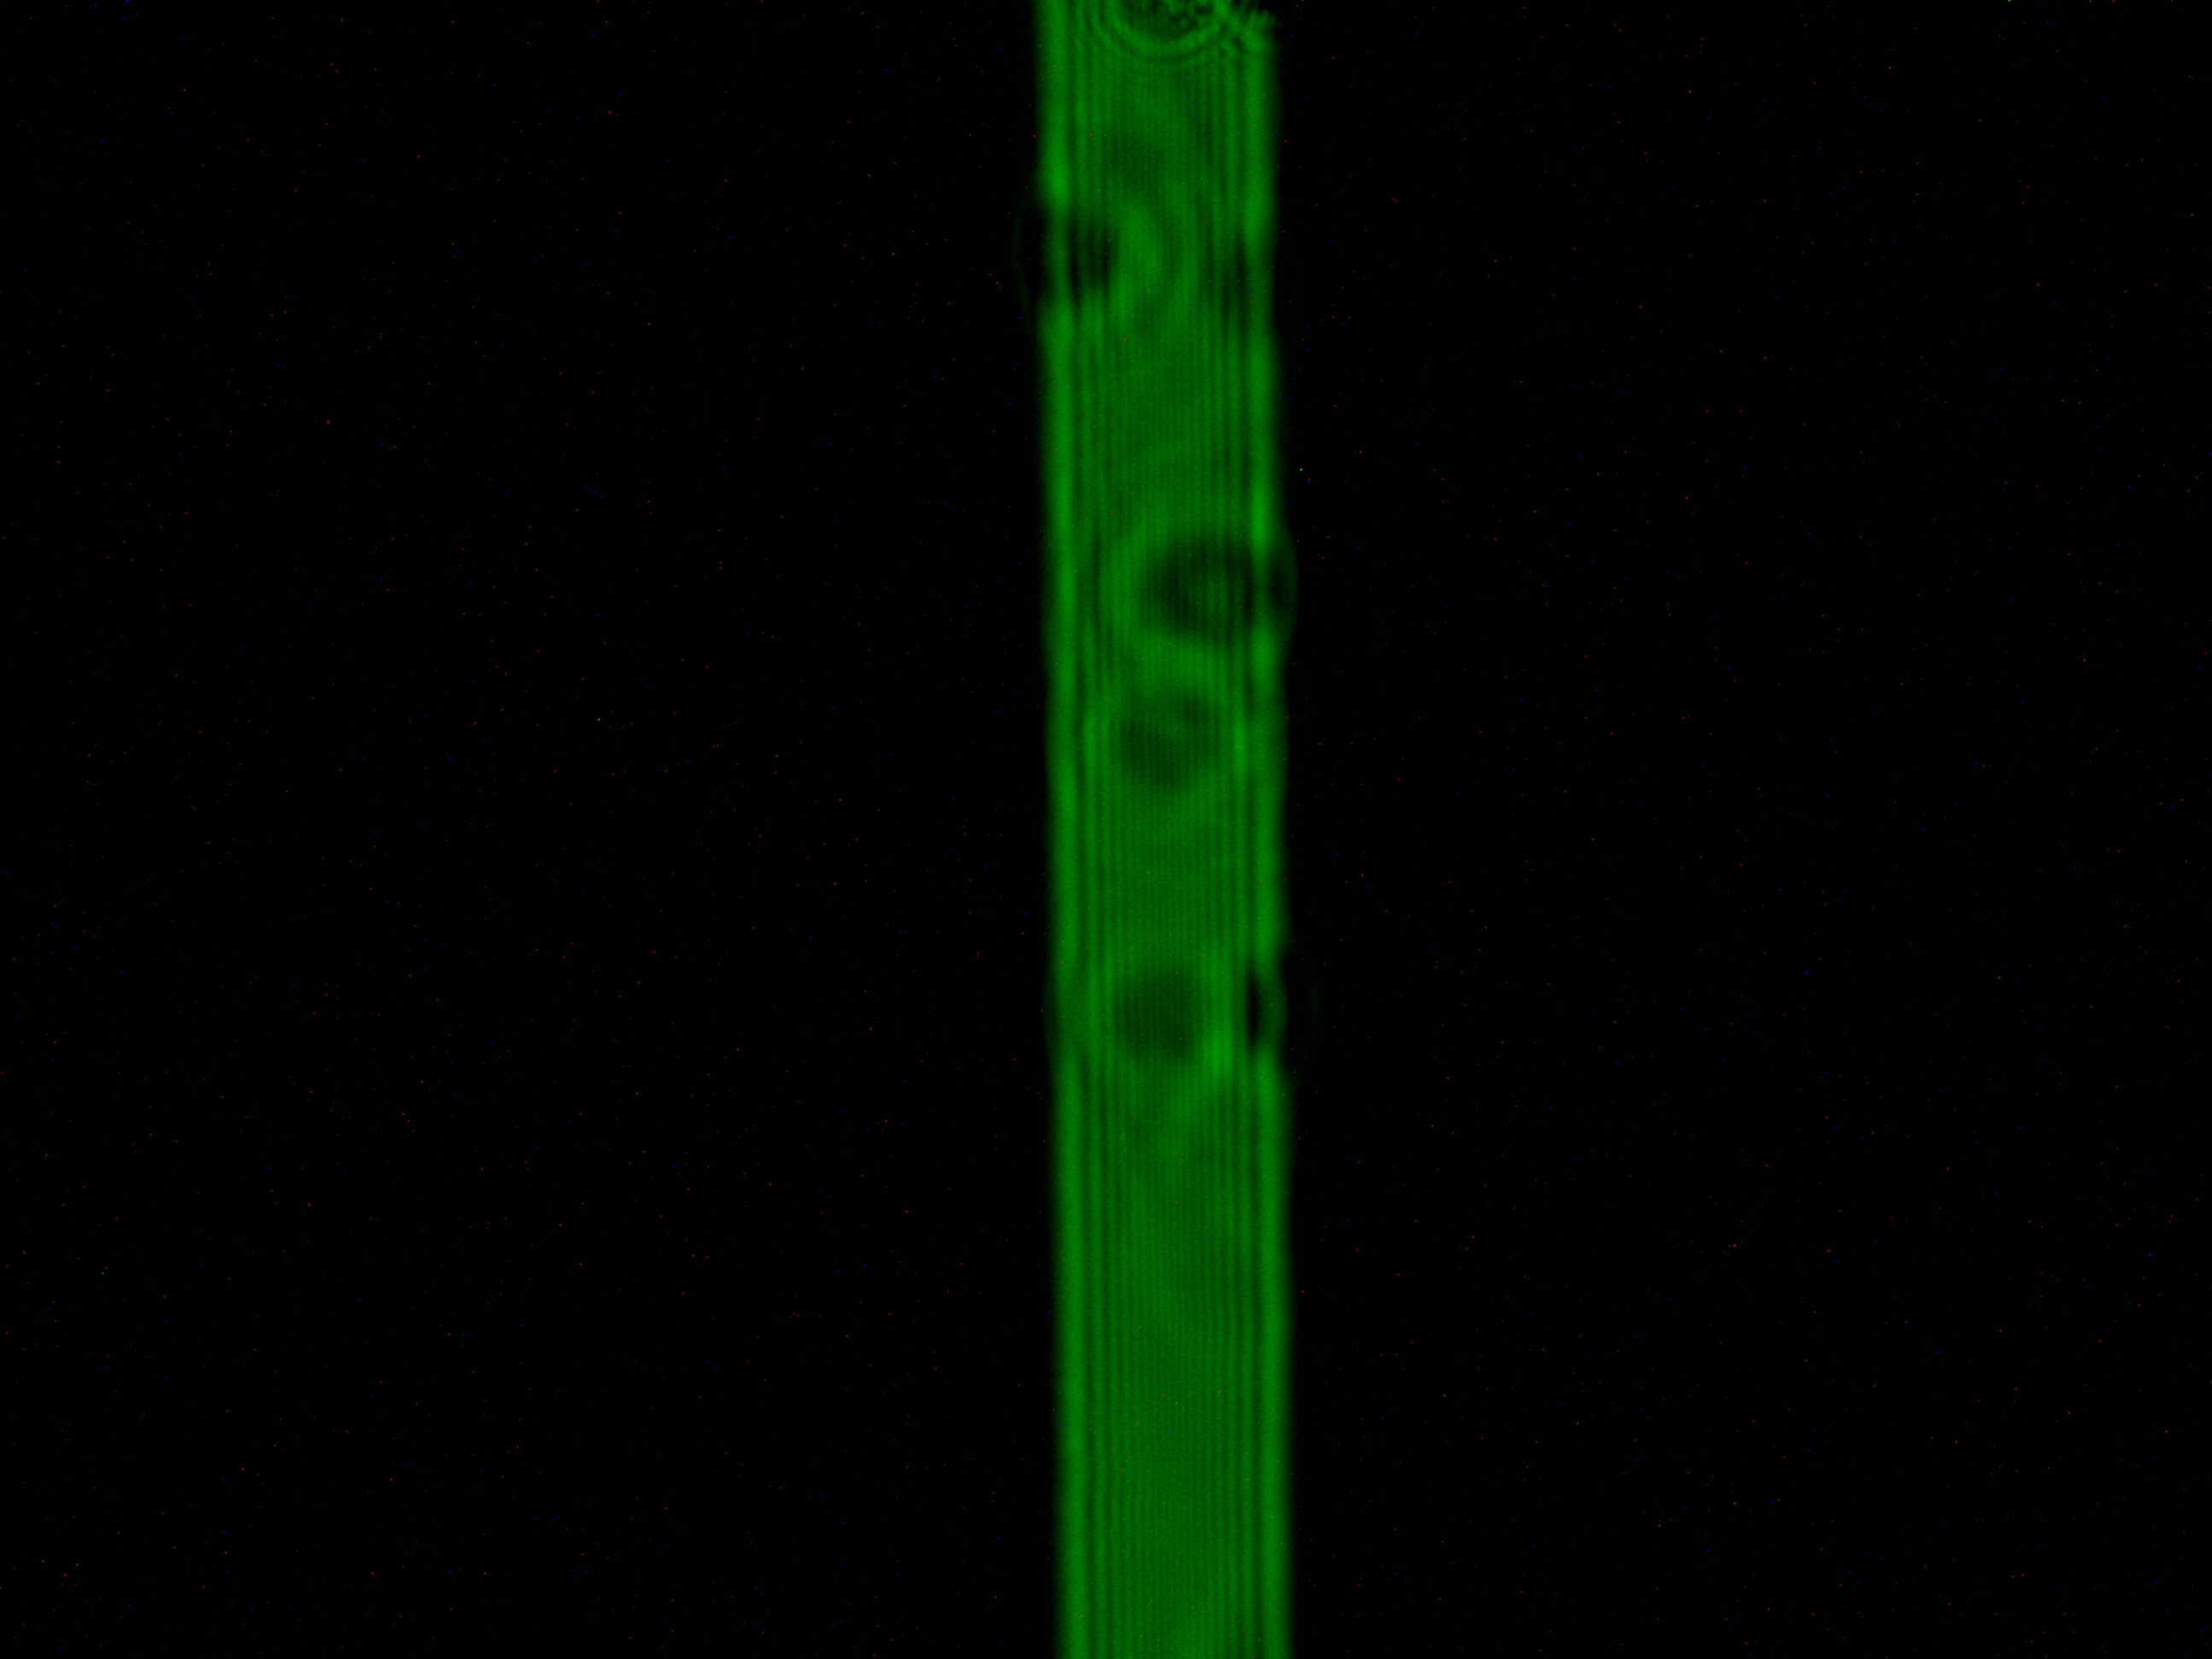
\includegraphics[width=\textwidth]{Фото/1.12.jpg}
        \caption{$d_2$ открыта поуже.}
    \end{minipage}
\end{figure}

    \item При исследовании дифракции на препятствии (алюминиевая полоса шириной 100 или 200 мкм) при удалении микроскопа наблюдалось чётное число тёмных дифракционных полос, а центр оставалься светлым:% что согласуется с теорией:

    \begin{figure}[H]
    \centering
    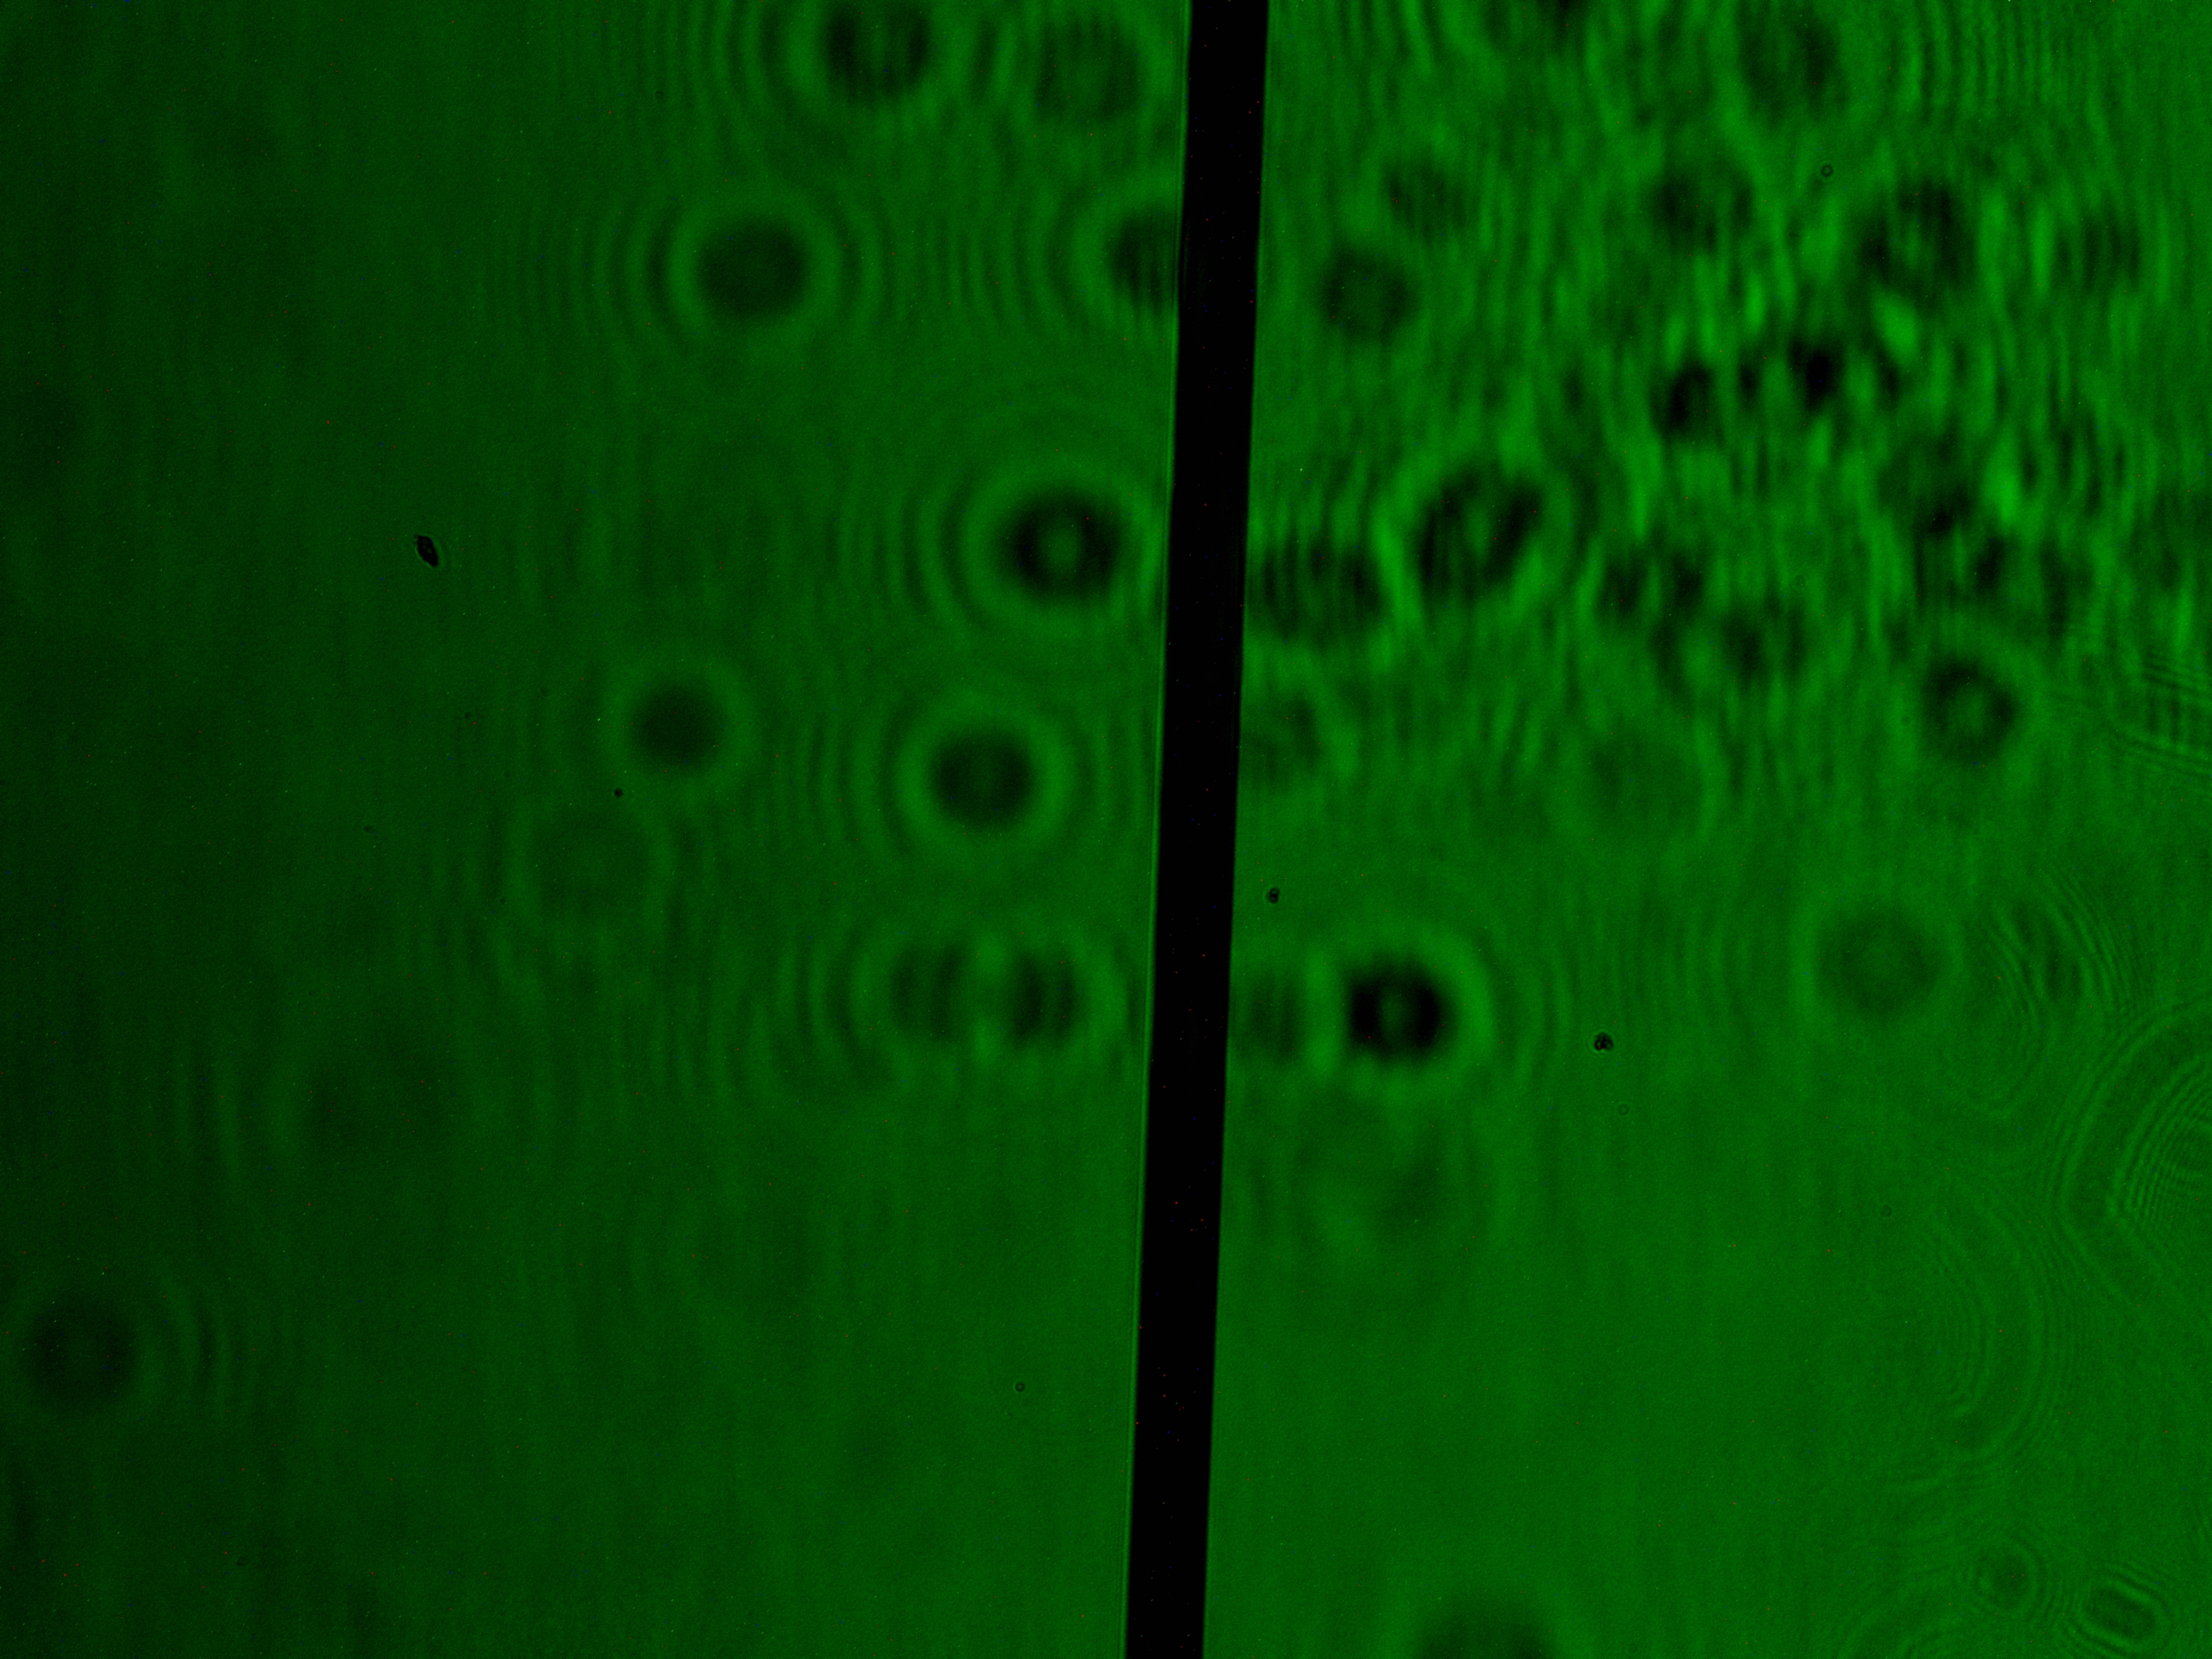
\includegraphics[width=0.5\textwidth]{Фото/1.13.jpg}
    \caption{Алюминиевая полоса при фокусировке на ней.}
\end{figure}
    \begin{figure}[H]
    \centering
    \begin{minipage}{0.45\textwidth}
        \centering
        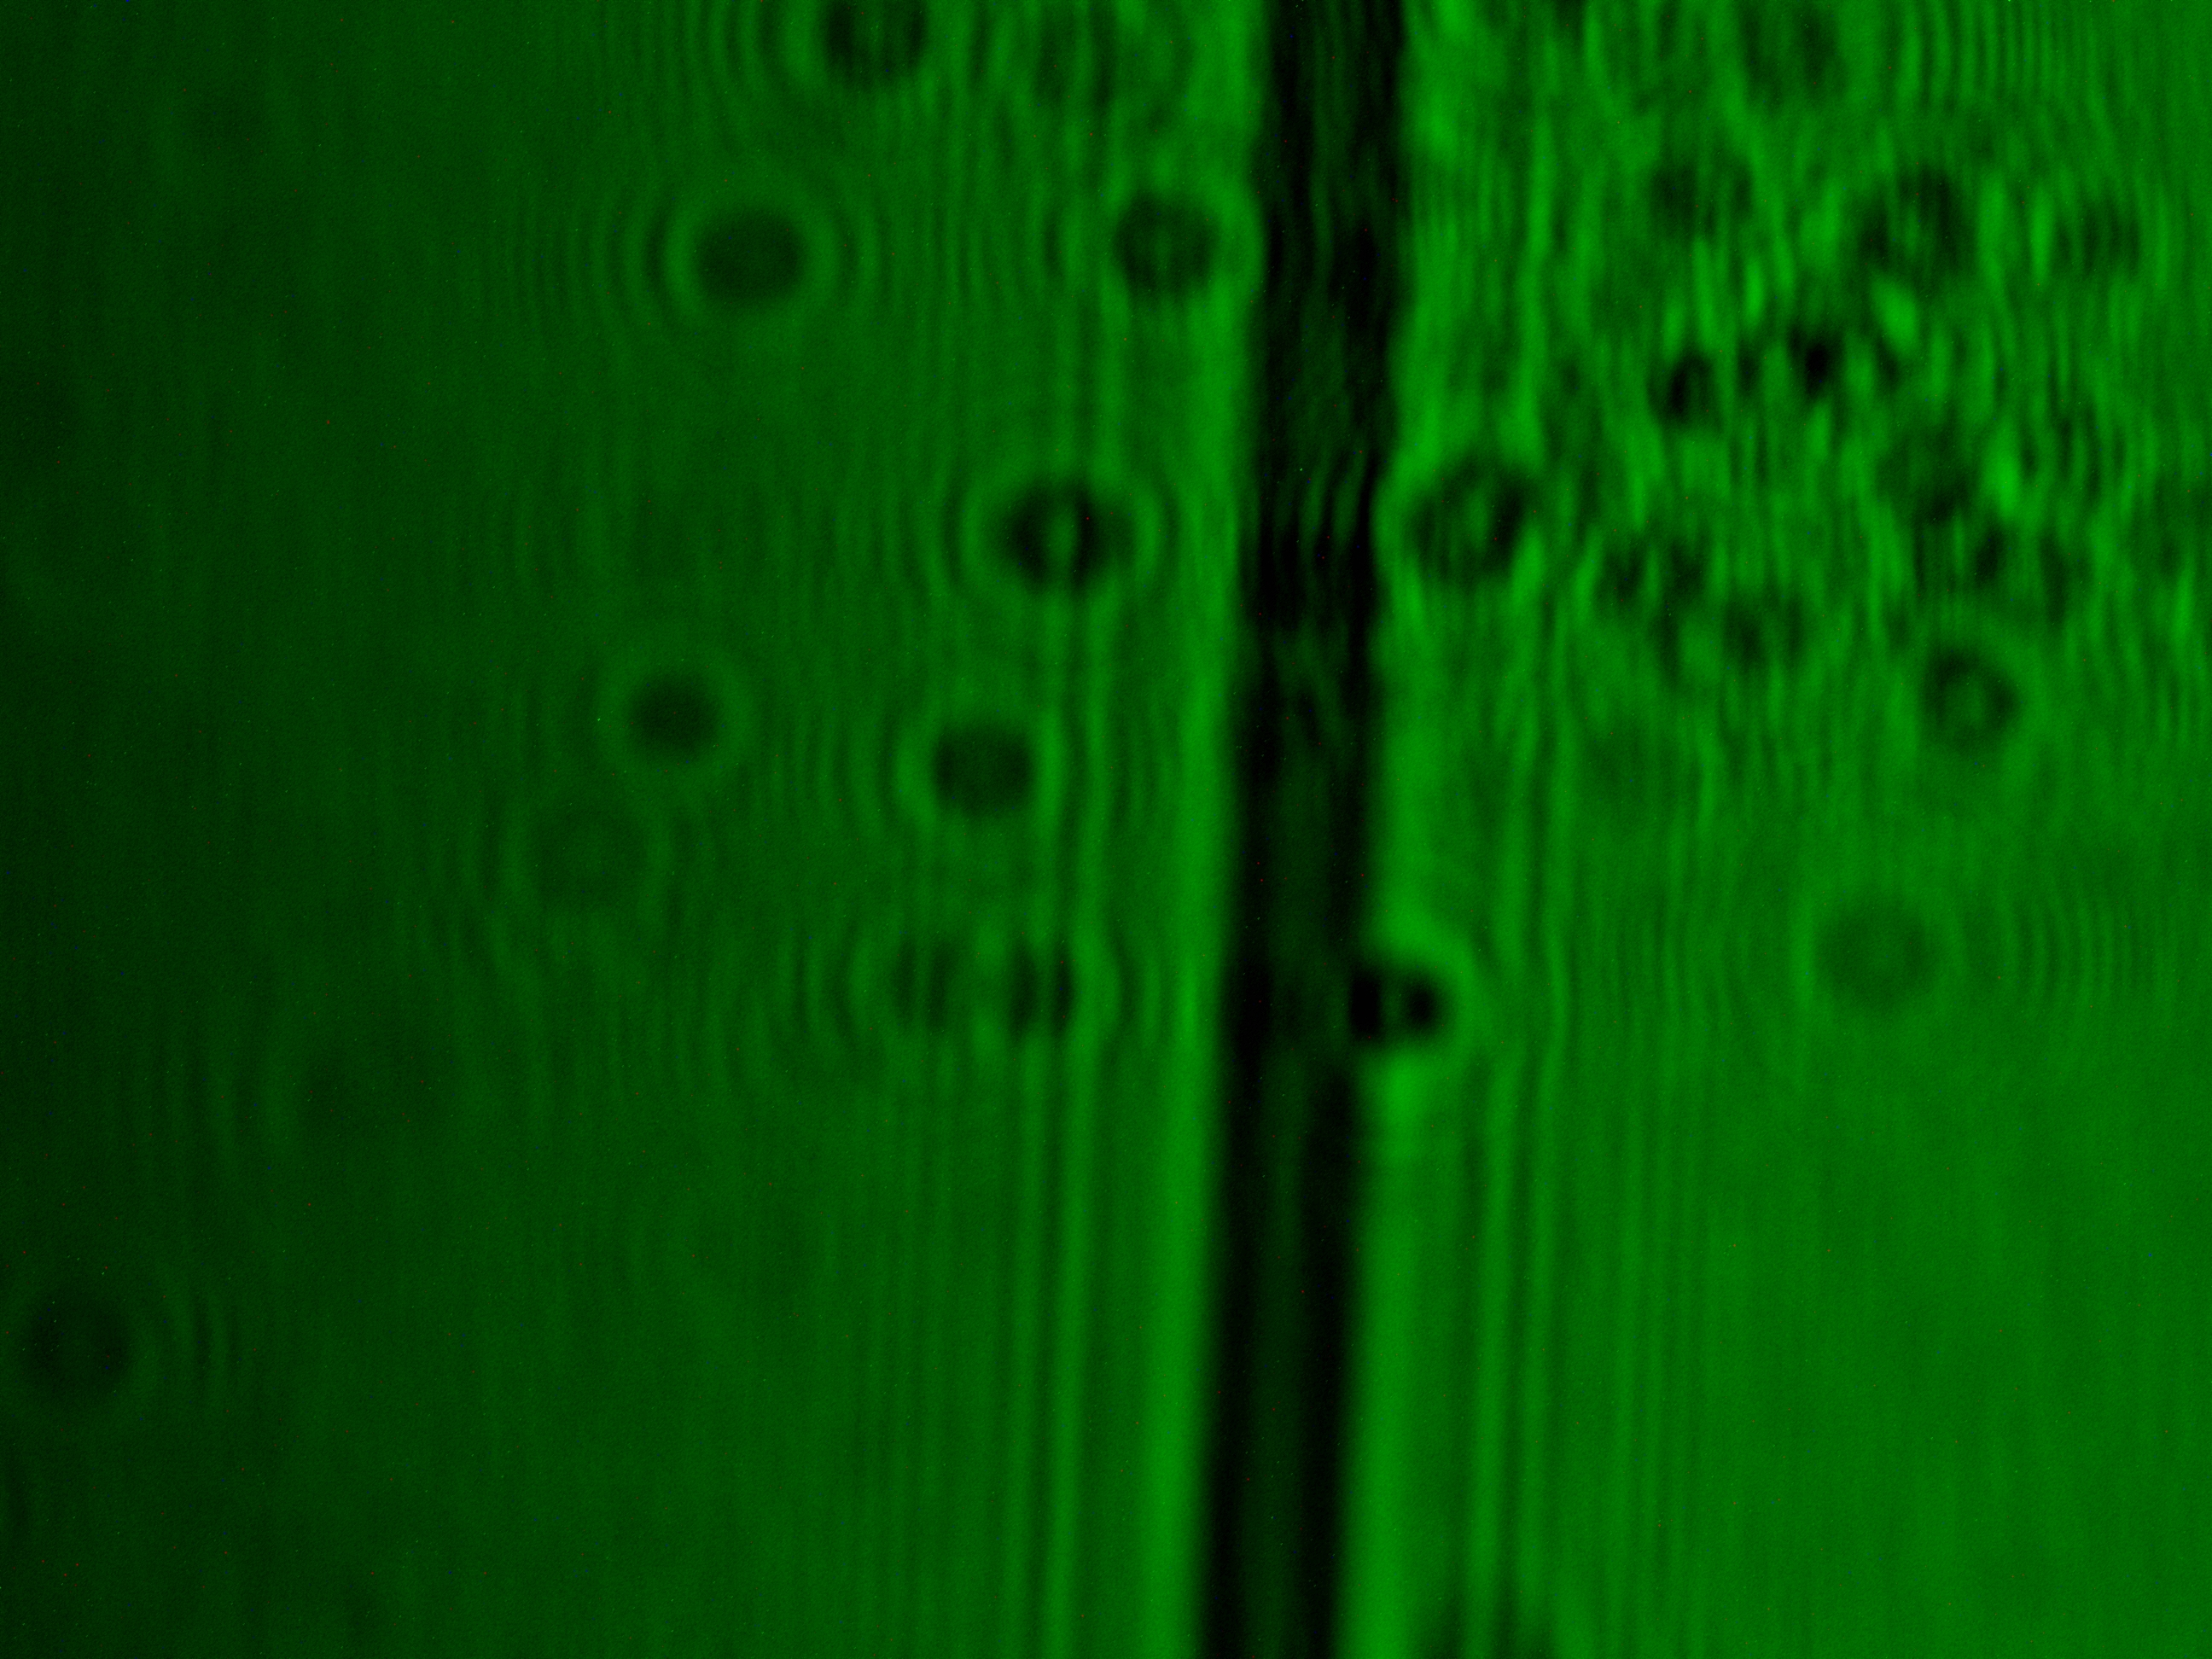
\includegraphics[width=\textwidth]{Фото/1.13 а.jpg}
        \caption{Алюминиевая полоса при небольшом отдалении.}
    \end{minipage}\hfill
    \begin{minipage}{0.45\textwidth}
        \centering
        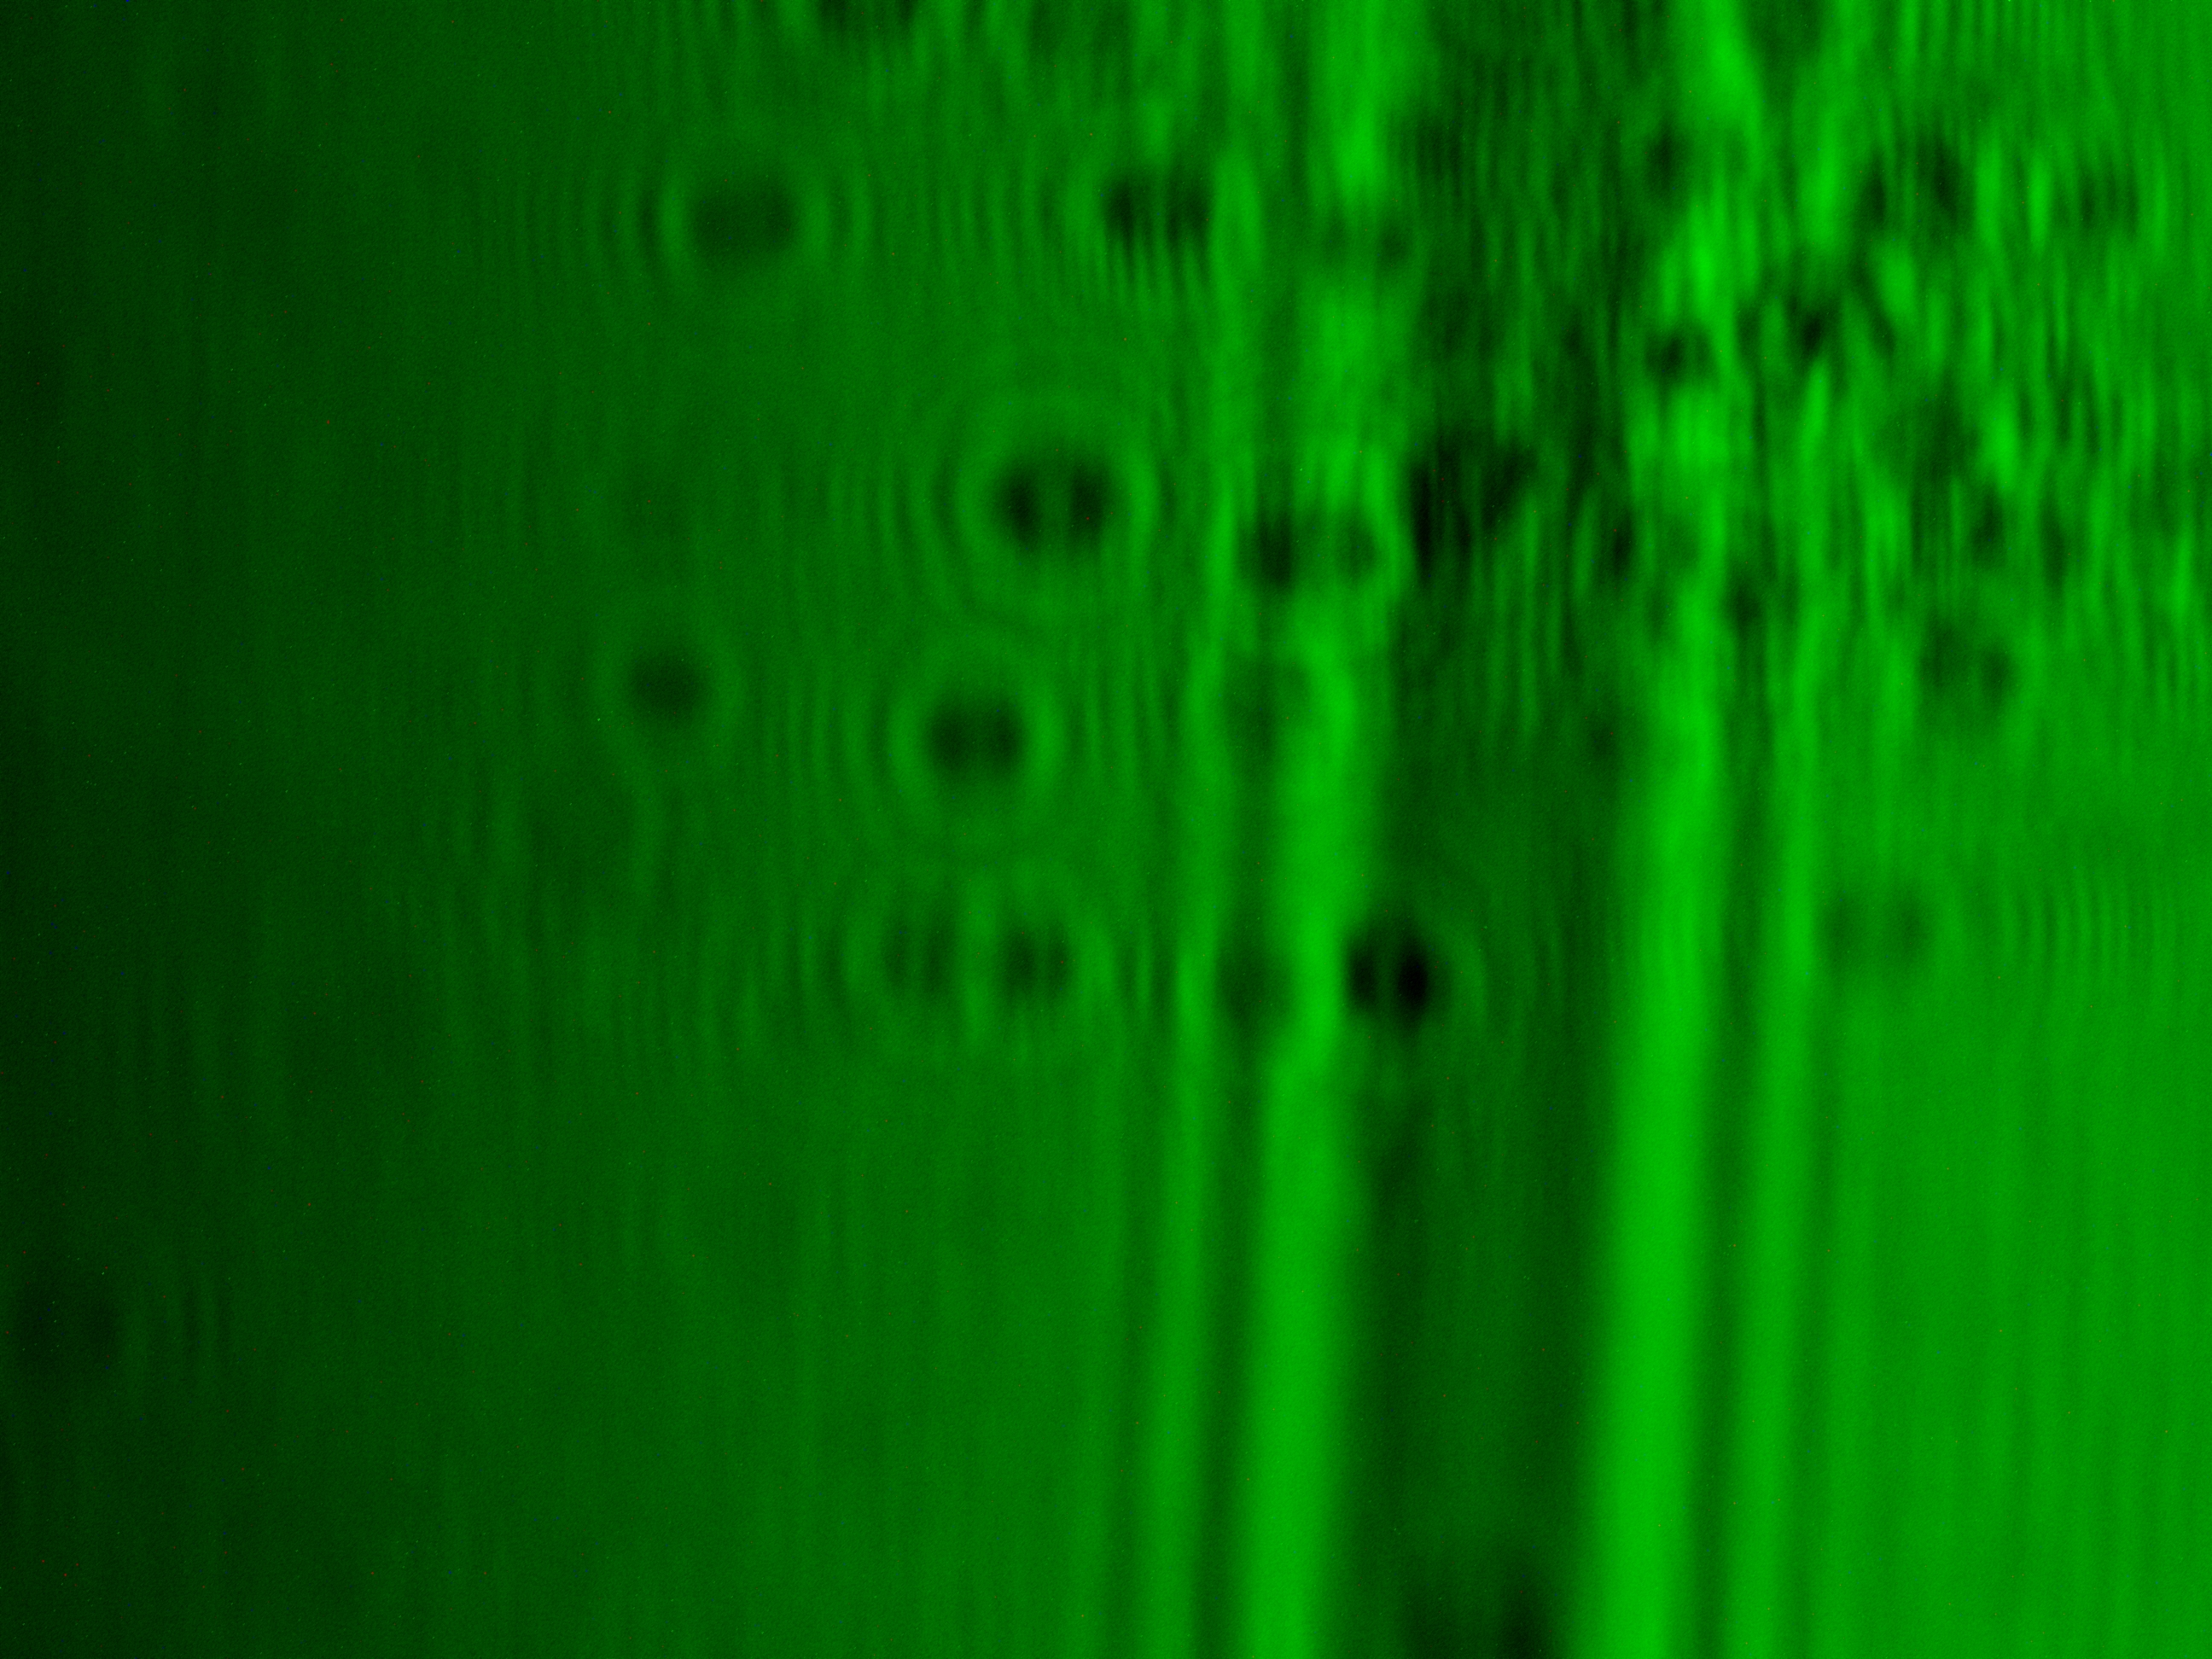
\includegraphics[width=\textwidth]{Фото/1.13 б.jpg}
        \caption{Алюминиевая полоса при большом отдалении.}
    \end{minipage}
\end{figure}
\end{itemize}












\subsection*{II. Дифракция Фраунгофера на щели}

Оптическая схема была перестроена согласно рис. 12. Положение источника света $S$, щели $d_1$ и линзы $l_1$ осталось без изменений. Щель $d_2$ была установлена вплотную к линзе $l_1$, а линза $l_2$ -- между $d_2$ и микроскопом. Сам микроскоп был настроен на фокальную плоскость $P$ линзы $l_2$.% Ширина щели $d_2$ была подобрана таким образом, чтобы дифракционная картина Фраунгофера заняла всё поле зрения микроскопа. Контрастность картины была оптимизирована уменьшением ширины входной щели $d_1$ и регулировкой интенсивности источника.

\begin{figure}[H]
    \centering
    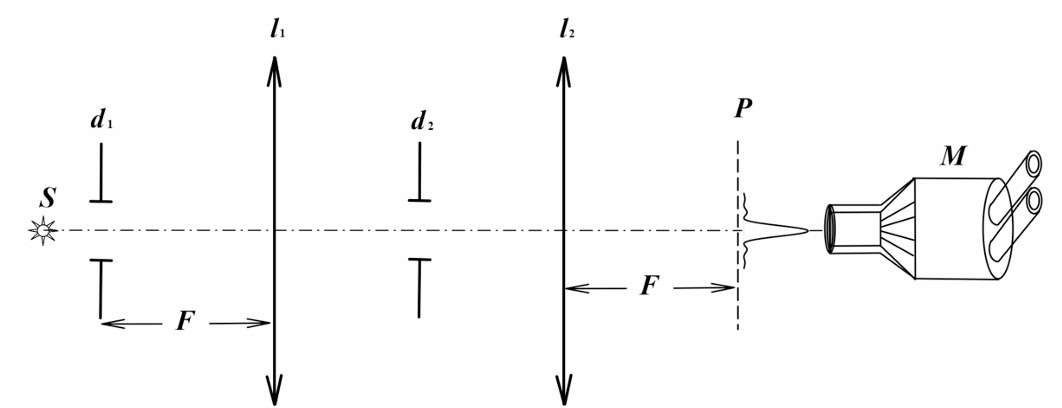
\includegraphics[width=0.5\textwidth]{5.jpg}
    \caption{Схема установки для наблюдения дифракции Фраунгофера на щели.}
\end{figure}

\textbf{Результаты измерений:}

Координаты $x_m$ дифракционных минимумов были измерены с помощью инструментов видеоокуляра в обе стороны от центрального максимума:

\begin{table}[H]
\centering
\begin{tabular}{|c|c|c|}
\hline
$m$ & $x_{\text{л}}$, мкм & $x_{\text{п}}$, мкм \\
\hline
1  & 91,07  & 92,37  \\\hline
2  & 179,53 & 179,53 \\\hline
3  & 269,30 & 268,00 \\\hline
4  & 357,76 & 353,86 \\\hline
5  & 450,13 & 444,93 \\\hline
6  & 534,69 & 534,69 \\\hline
7  & 624,46 & 624,46 \\\hline
8  & 714,22 & 712,92 \\\hline
9  & 805,29 & 800,09 \\\hline
10 & 892,45 & ---    \\
\hline
\end{tabular}
\caption{Положения дифракционных минимумов}
\end{table}

Ширина щели (определена с помощью микроскопа): $d_{2\text{}} = (881\pm 5)$ мкм.



% \textbf{Обработка результатов:}

Построен график зависимости положений экстремумов $x_m$ от их номера $m$:

\begin{figure}[H]
    \centering
    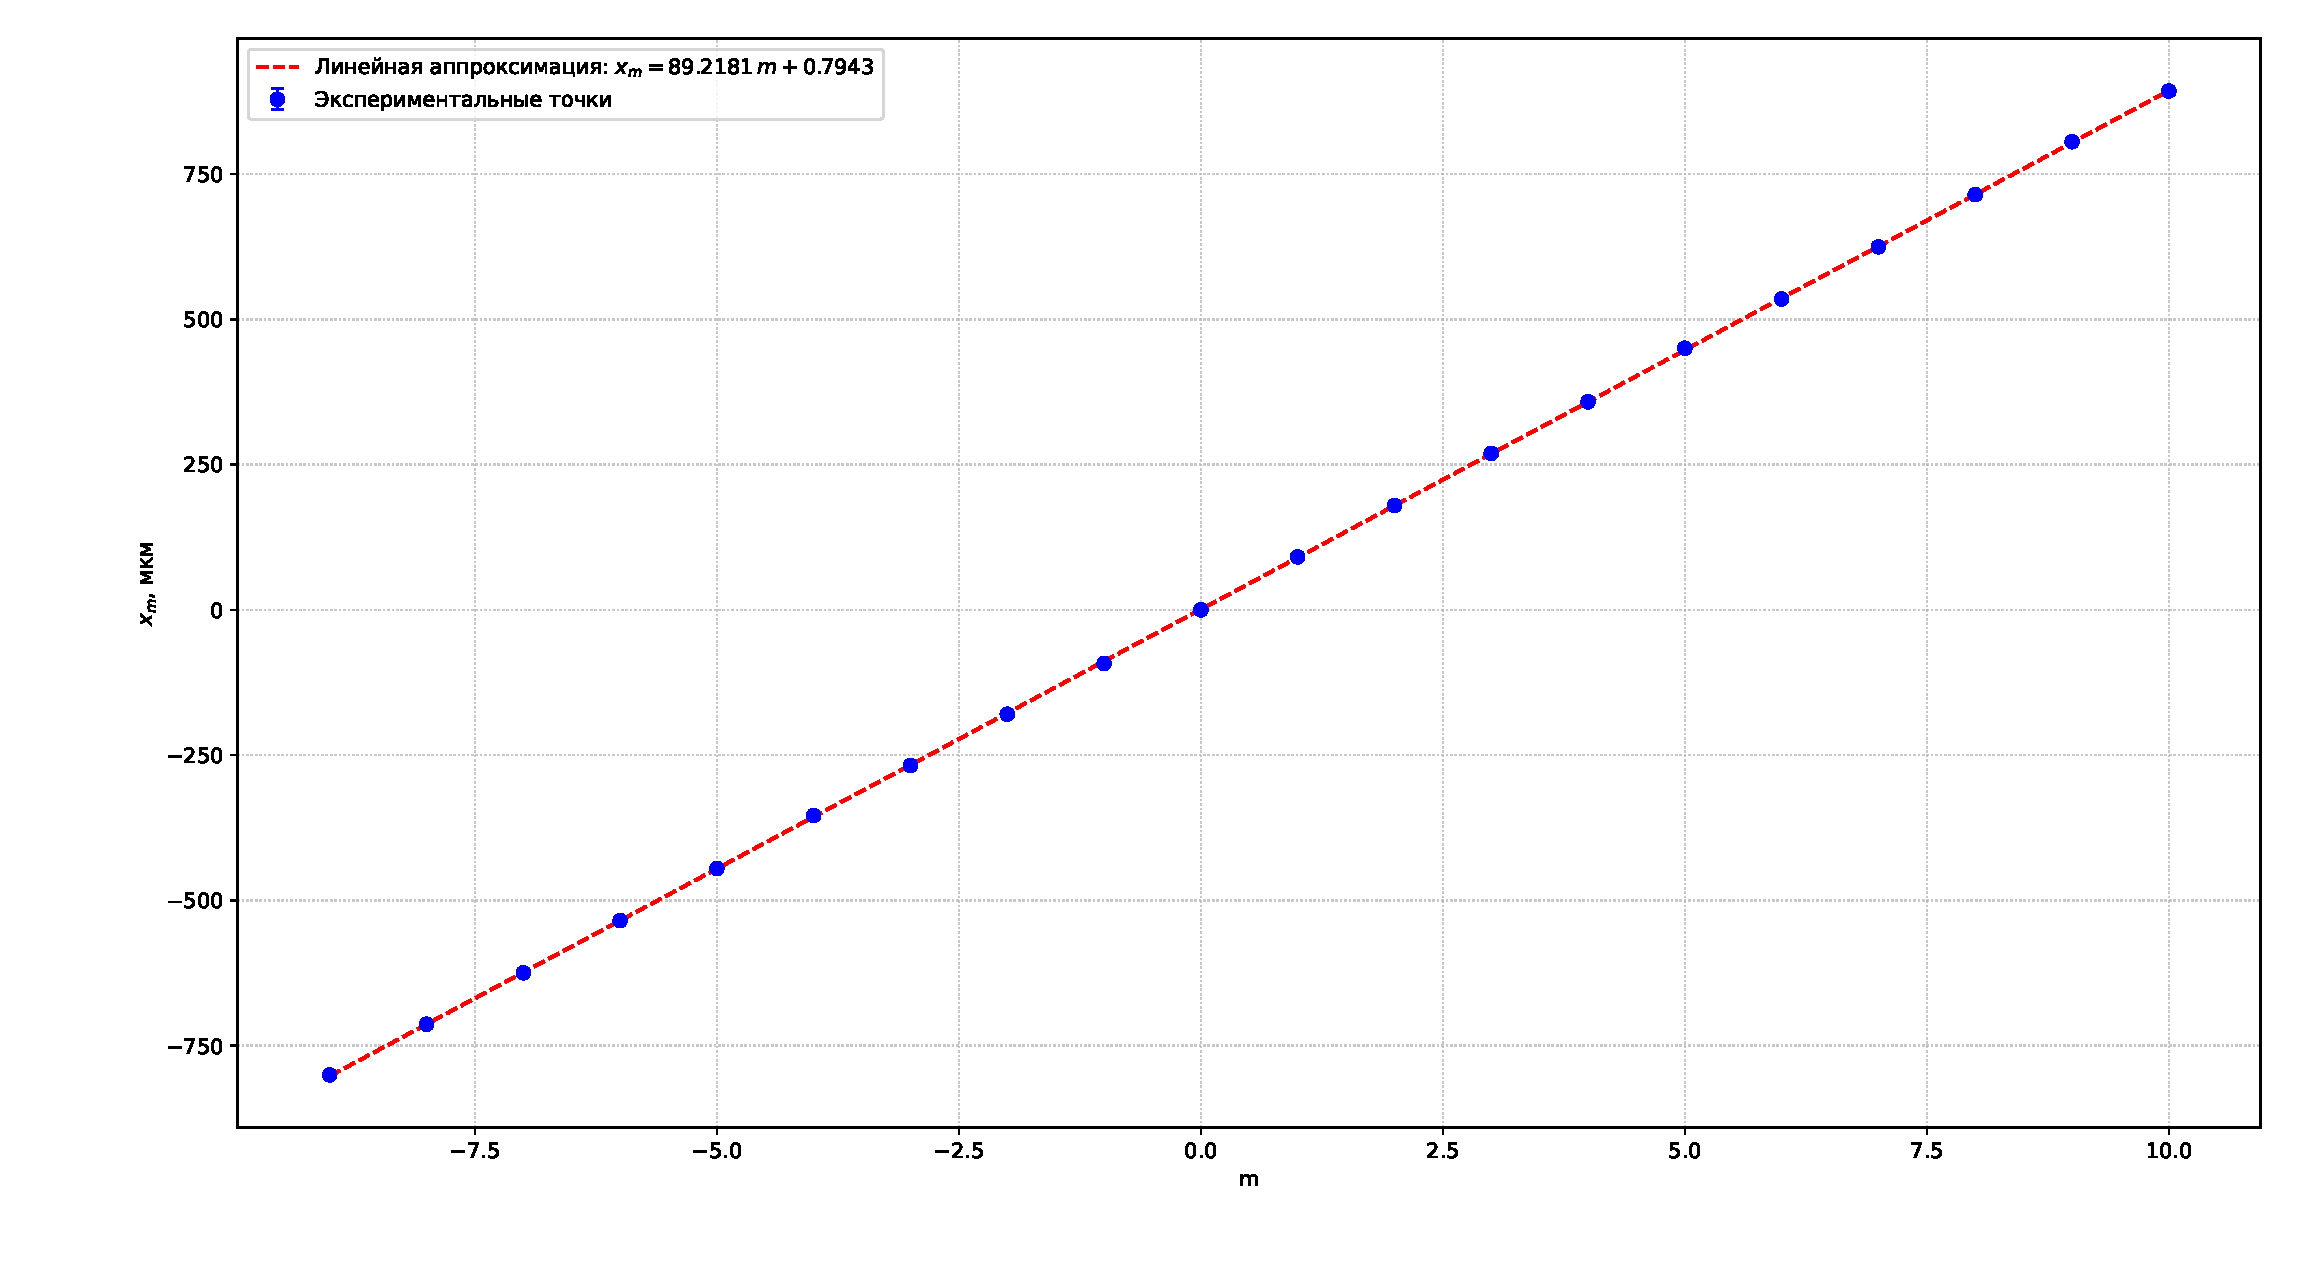
\includegraphics[width=0.8\textwidth]{xm.pdf}
    \caption{Зависимость положений минимумов $x_m$ от номера $m$}
    \label{fig:fraunhofer_xm}
\end{figure}

Экспериментальная зависимость аппроксимирована прямой, по наклону графика из формулы $x_m = f \dfrac{m \lambda}{d}$ была определена ширина щели:
$$d_{2} = (1119,7 \pm 13) \text{ мкм}$$

(где $f = 18$ см -- фокусное расстояние линзы $l_2$, $\lambda = 555$ нм).


% Полученные результаты подтверждают справедливость формулы для координат минимумов при дифракции Фраунгофера: $x_m = f \cdot m\lambda / b$.
\textbf{Качественные наблюдения:}

\begin{itemize}
    \item Смещение щели $d_2$ в боковом направлении не приводило к сдвигу дифракционной картины. Это объясняется тем, что при нормальном падении плоской волны угловое распределение интенсивности определяется только геометрией щели и не зависит от её положения в поперечном направлении.
    
    \item При уменьшении ширины щели $d_2$ наблюдалось увеличение масштаба (расширение) дифракционной картины, что следует из теоретической зависимости $x_m \propto 1/b$.
\end{itemize}

\begin{figure}[H]
    \centering
    \begin{minipage}{0.45\textwidth}
        \centering
        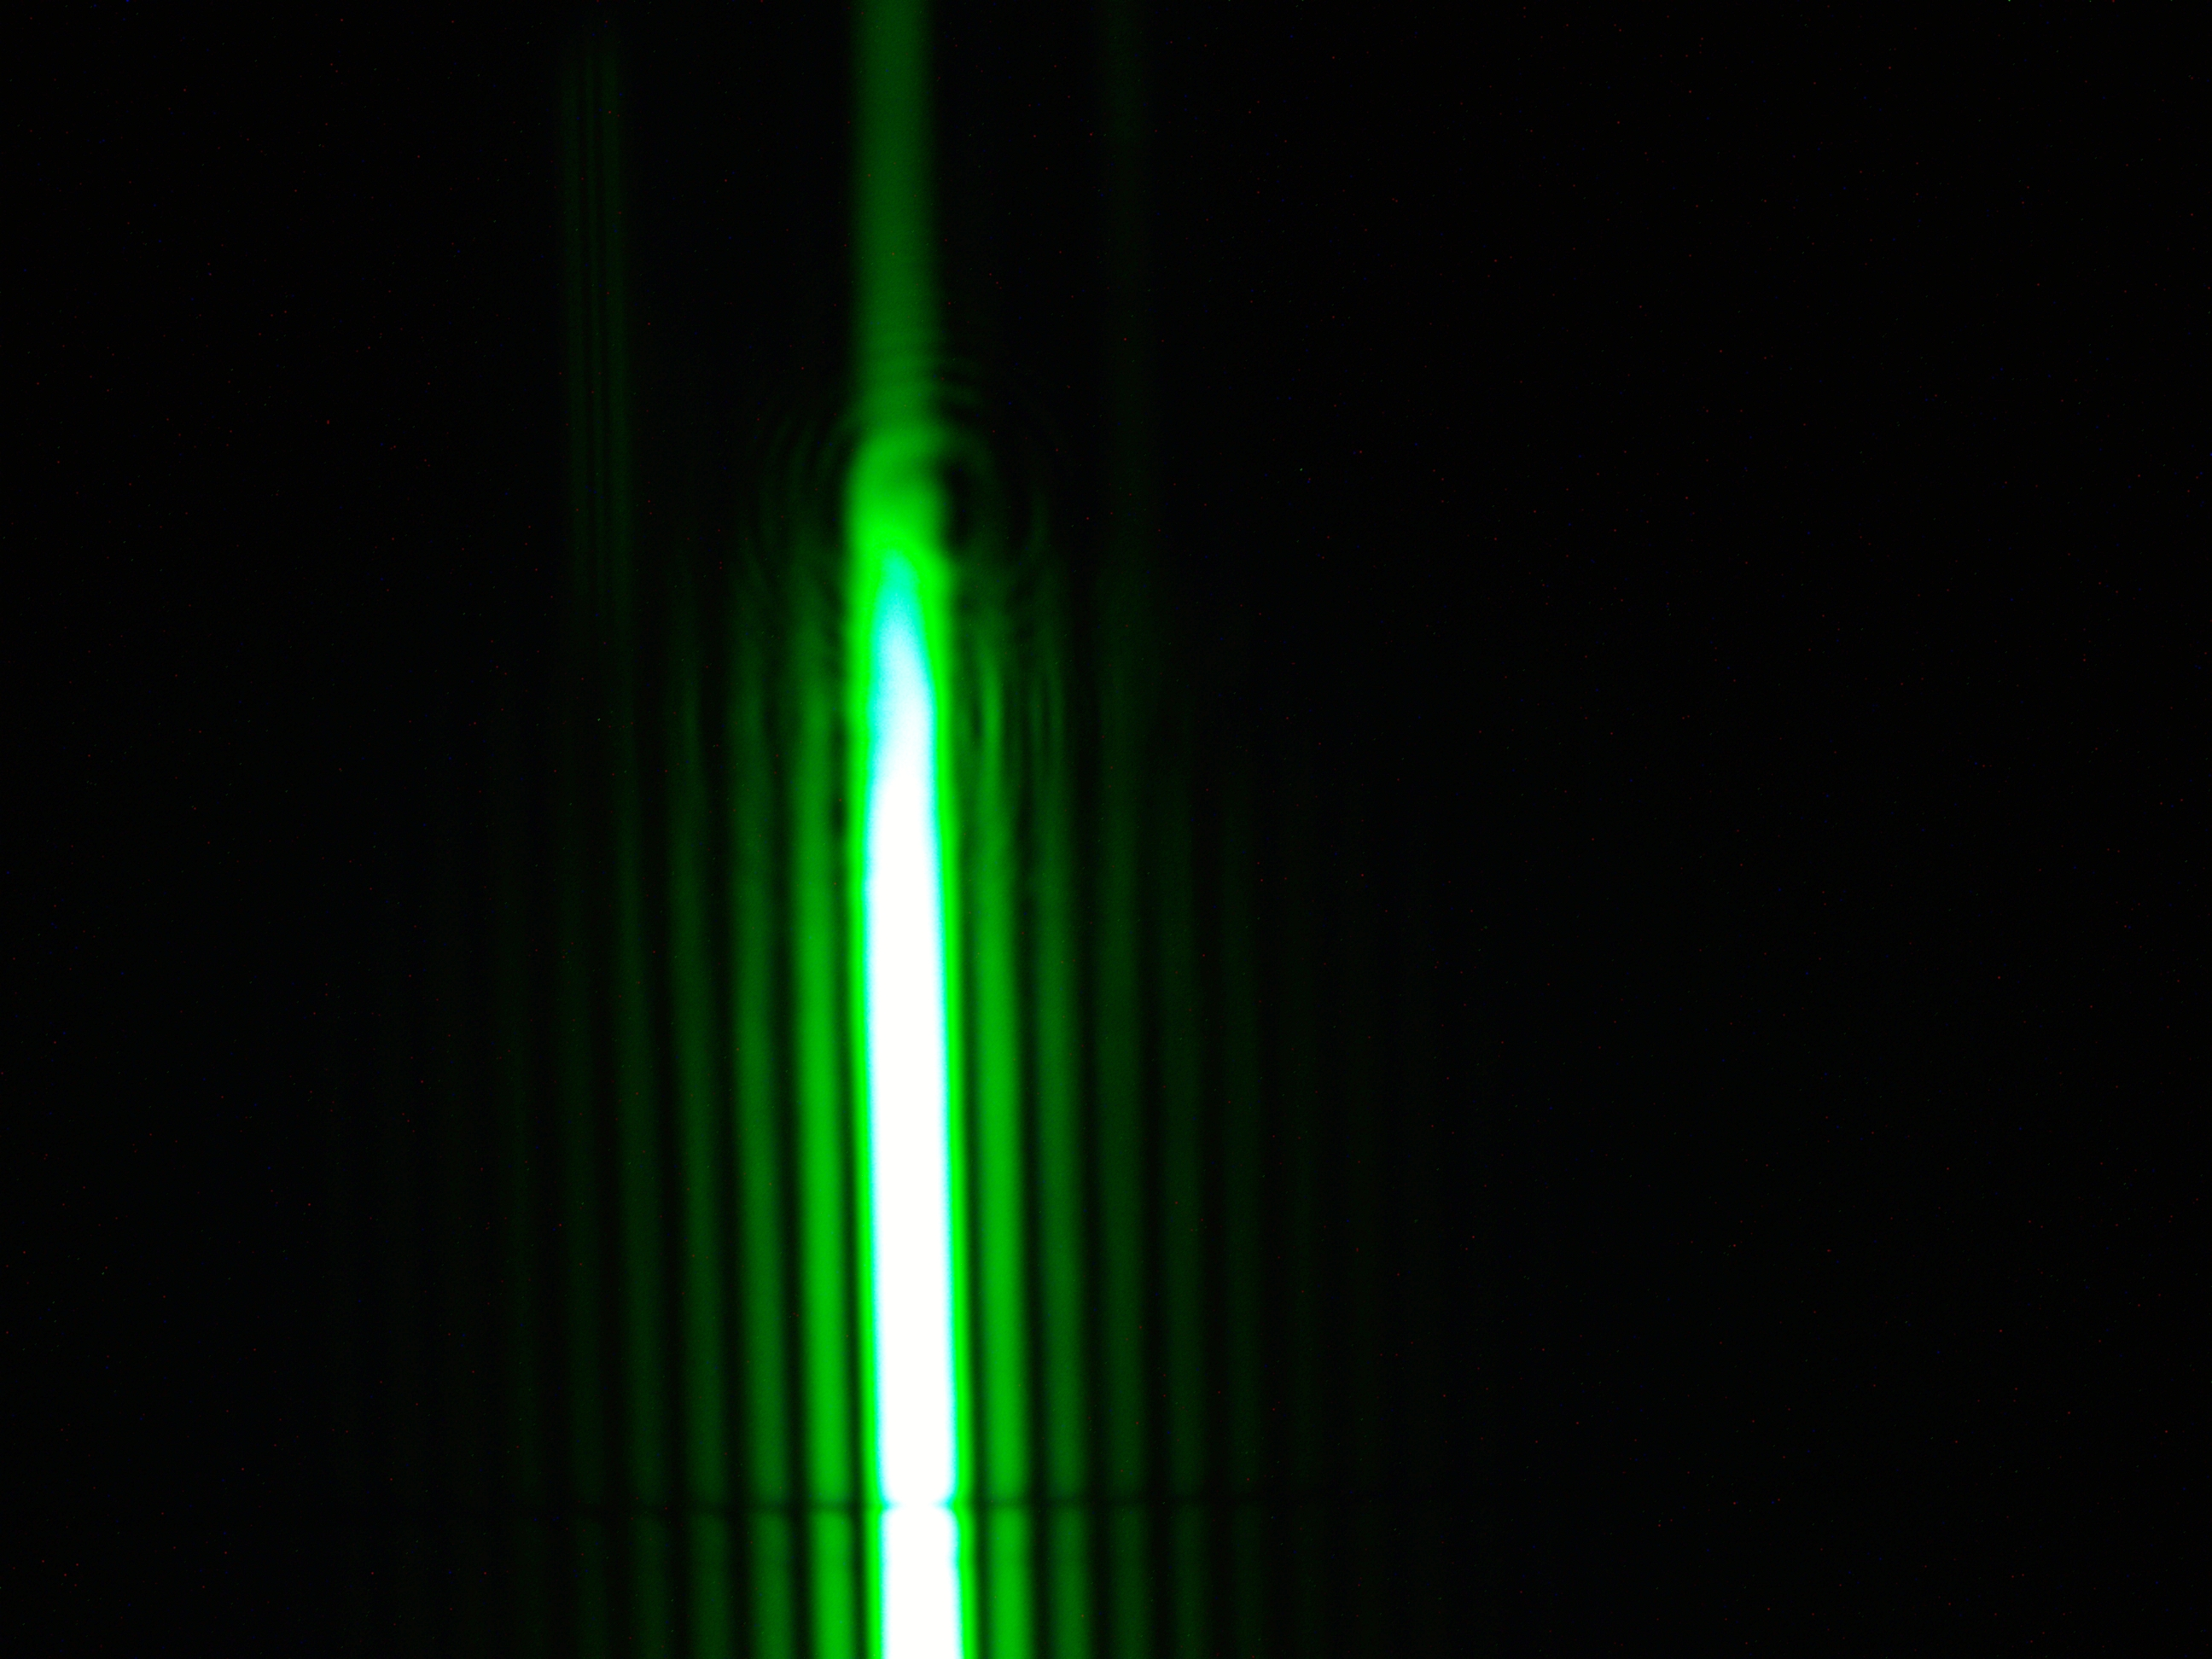
\includegraphics[width=\textwidth]{Фото/2.8 широко.jpg}
        \caption{Картина при более широкой щели.}
    \end{minipage}\hfill
    \begin{minipage}{0.45\textwidth}
        \centering
        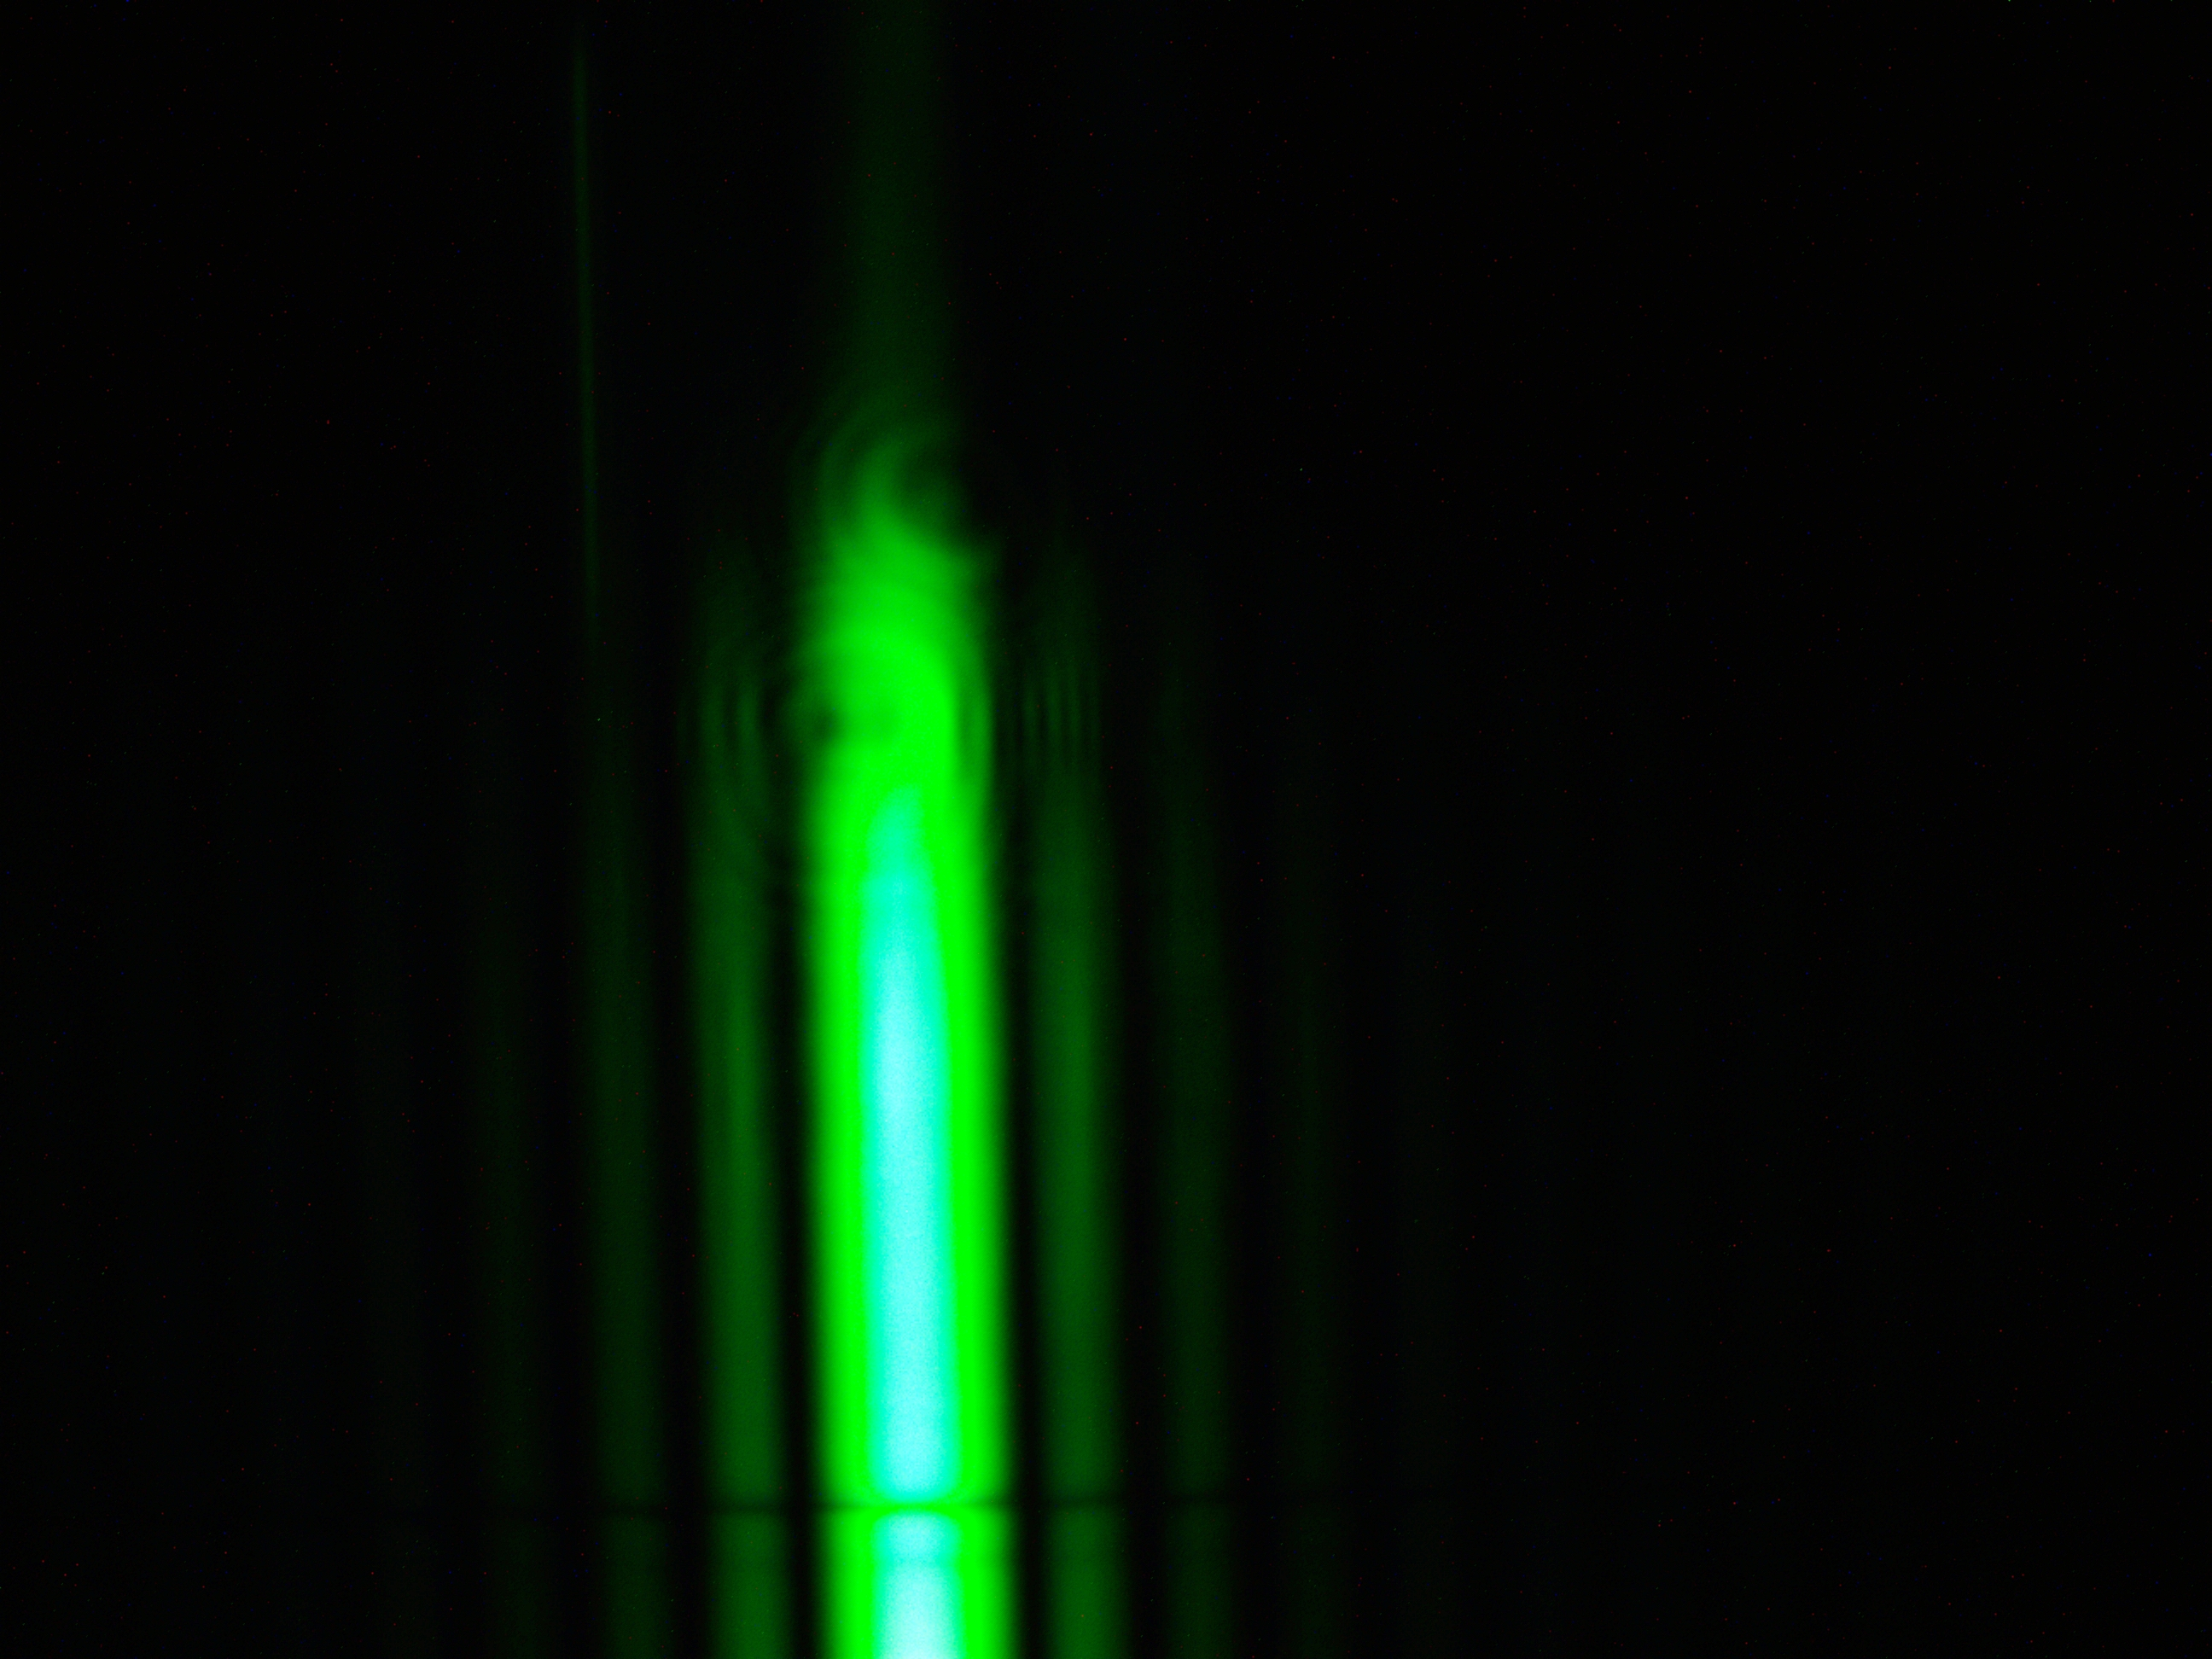
\includegraphics[width=\textwidth]{Фото/2.8 узко.jpg}
        \caption{Картина при более узкой щели.}
    \end{minipage}
\end{figure}

\section*{Вывод}

В ходе выполнения лабораторной работы были экспериментально исследованы дифракционные явления в ближней и дальней волновых зонах.

При изучении дифракции Френеля на щели зависимость координаты дифракционного минимума от его порядка была аппроксимирована линейной функцией, что подтвердило справедливость метода зон. Ширина щели, определённая по наклону графика ($b_{\text{граф}} = 403$ мкм), не совпала с прямым измерением ($b_{\text{экр}} = 475,7$ мкм), поскольку нам не была в точности известна длина волны светодиода.% С помощью спирали Корню было показано, что интенсивность на самой границе геометрической тени составляет одну четверть от интенсивности вдали от экрана в освещённой области, так как амплитуда колебаний на краю соответствует половине вектора для полностью открытого фронта. При замене щели на непрозрачное препятствие наблюдался светлый центр дифракционной картины, что подтвердило принцип Бабине.

При исследовании дифракции Фраунгофера было подтверждено линейное соотношение между координатами минимумов $x_m$ и их номером $m$: $x_m = f \cdot m\lambda / b$. Угловая ширина центрального максимума оказалась обратно пропорциональна ширине щели. Ширина щели, определённая по наклону графика $x_m(m)$ ($b_{\text{граф}} = 1119,7$ мкм), не совпала с определённой с помощью микроскопа ($b_{\text{экр}} = 881$ мкм) также из-за неизвестности точных значений длины волны светодиода и фокусного расстояния линзы.

% Таким образом, теоретические модели дифракции Френеля и Фраунгофера, основанные на принципе Гюйгенса-Френеля и методах векторных диаграмм (спирали Френеля и Корню), были успешно верифицированы экспериментально. Все наблюдаемые явления согласовались с предсказаниями волновой оптики.

\end{document}